\documentclass[10pt]{article}
\usepackage{parskip}
\usepackage[utf8]{inputenc}
\usepackage[left=2.00cm, right=2.00cm, top=2.00cm, bottom=2.00cm]{geometry}
\usepackage[spanish]{babel}
\usepackage{graphicx,subfig}
\usepackage{fancyhdr}
\graphicspath{{Imagenes/}}
\usepackage{enumerate} 
\usepackage{multicol}
<<<<<<< HEAD
\usepackage{tabularx}
=======
\usepackage{amssymb}
\usepackage{adjustbox}
\usepackage{amsmath}
\usepackage{cancel}
>>>>>>> 05e24634aa0090a7e477c33ffea4fc7ff62d4b5e
\begin{document}


\pagestyle{fancy}
\cfoot{}


%Cabeceras
\rhead{Multímetro.}
\lhead{}

%Portada
\begin{titlepage}
	\newgeometry{
		left=25mm,
		right=25mm,
		top=5mm,
		bottom=30mm,
		headheight = 0 mm
	}

	\begin{figure}[t]
		\subfloat{
\includegraphics[width=0.15\textwidth]{Logo_IPN}}
		\hspace{0.6\textwidth}
		\subfloat{
\includegraphics[width=0.22\textwidth]{LogoEsime}}
	\end{figure}

	\centering
	{\bfseries\Huge Instituto Politécnico Nacional. \par}
	\vspace{1cm}
	{\scshape\Large Ingeniería en Comunicaciones y Electrónica. \par}
	\vspace{0.3cm}
	{\scshape\Large Laboratorio de Electricidad y Magnetismo.  \par}
	\vspace{1cm}
	{\scshape\Huge El Universo de las Mediciones Eléctricas. \par}
	\vspace{1cm}
	{\itshape\Large Multímetro. \par}
	{\Large 2CM13\par}
	\vfill
	{\Large Autores: \par}
	{\Large Daniela Elizabeth Pérez Vargas. \par}
	{\Large Jesús Martinez Amac. \par}
	{\Large José Emilio Hernández Huerta. \par}
	{\Large Nataly Bejarano Garduño.\par}
	{\Large Uriel Grimaldi Díaz.  \par}
	\vfill
	{\Large Mayo 2023. \par}

\end{titlepage}

\tableofcontents
\newpage

\section{Resumen.}
En la presente práctica, se desarrolla el uso del multímetro con enfásis en las funciones de medición de resistencia, continuidad, diferencia de potencial eléctrico (en Corriente Directa y Corriente Alterna) y corriente eléctrica. 

\begin{multicols}{2}

\section{Objetivo.}

El alumno será capaz de describir las características y funcionamiento del multímetro así como manejar correctamente dicho instrumento para realizar mediciones de las 3 magnitudes eléctricas fundamentales (Resistencia, diferencia de potencial eléctrico y corriente eléctrica).

\section{Introducción.}

La herramienta fundamental del técnico o ingeniero especializado en la manipulación de componentes electrónicos es el multímetro, dicha herramienta permite al profesional obtener mediciones de magnitudes eléctricas que le puedan resultar útiles,
estas magnitudes suelen ser , la resistencia eléctrica, la diferencia de potencial eléctrico, la corriente eléctrica,frecuencia, inductancia, capacitancia además de otras utilidades como la continuidad y la prueba de diodos.

\section{Marco teórico.}

\subsection{El multímetro.}
Se denomina multimetro al instrumento que es capaz de realizar las funciones de voltímetro, amperímetro y óhmetro. Los multimetros digitales suelen incorporar funciones adicionales como capacítometro, frecuenciometro, medida de hfe (ganancia) de transistores, para medir 
temperaturas sobre superficies además de otras utilidades como la continuidad eléctrica y la prueba de diodos.

Con los multímetros digitales no solo es posible realizar medidas de diferencia de potencial eléctrico y de corrientes continuas, si no que también nos permiten medir el diferencia de potencial eléctrico de corrientes alternas.

Un multímetro está formado por distintos bloques funcionales que forman las <<etapas>> de tratamiento de la señal a medir.

\begin{center}
	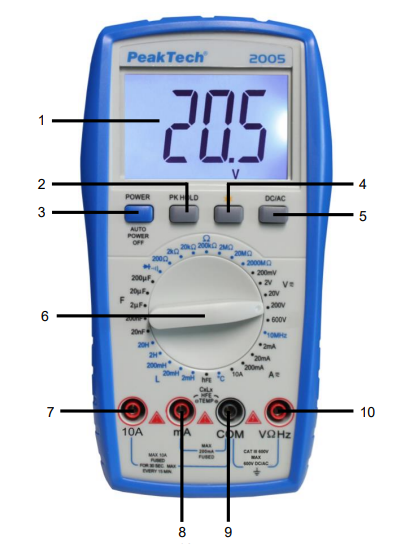
\includegraphics[scale = 0.5]{Imagenes/Marco/Multimetro.PNG}\\
	\begin{enumerate}
		\item Pantalla LCD
		\item Tecla PK Hold.
		\item Tecla de encendido y apagado.
		\item Tecla de retroiluminación.
		\item Tecla Corriente Directa / Corriente Alterna.
		\item Selector.
		\item Conector de entrada 10 A.
		\item Conector de entrada mA/temp.
		\item Conector de entrada COM.
		\item Conector de entrada V/$\Omega$/Hz.
	\end{enumerate}
\end{center}

Un consejo relevante cuando se usan instrumentos analógicos es que siempre conviene medir lo máximo posible el fondo de escala para reducir el error en la medición.

\subsection{Antes de usar un multímetro.}
Dentro de las comprobaciones de rutina tenemos , primeramente, asegurarnos de que el multímetro tenga buena carga de batería, una forma de saber si tiene una carga adecuada de batería si el multímetro no posee medidor de batería es hacer una prueba de continuidad, si el sonido
es débil es probable que el multímetro requiera de batería.

También tenemos que verificar que el fusible de protección del multímetro no esté cortado, generalmente este fusible se encuentra en la parte trasera del multímetro. Verificamos de igual manera que las puntas se encuentren en buenas condiciones y por último, una correcta medida se hace
sin tocar las puntas metalicas , solo sosteniendo las puntas de medición por su mango de plástico.

\subsection{Como utilizar el multímetro.}

A continuación se detallaran las recomendaciones e instrucciones para utilizar correctamente el multímetro para leer las 3 magnitudes fundamentales (Diferencia de potencial eléctrico,corriente y resistencia).
\subsubsection{Diferencia de potencial eléctrico.}

Siga las recomendaciones del manual de usuario sobre el máximo de Diferencia de potencial eléctrico soportado por su multimetro.
\begin{enumerate}
	\item Coloque el selector en la posición adecuada. Seleccione el rango según se necesite, si no conoce el valor apróximado a medir, inicie primero en la posición de mayor escala y vaya reduciendo según lo pida la lectura.
	\item Conecte la punta de medición negra a la terminal COM y la punta roja a la terminal V/$\Omega$/Hz.
	\item Conecte las puntas de medición a la fuente que desee medir.
\end{enumerate}

Como recomendación adicional, es importante no girar el selector a otro rango ya que podría dañar los componentes del medir.
\subsubsection{Corriente eléctrica.}

Primeramente se tiene que conectar el medidor en serie con el circuito.

Las terminales que permiten medir Corriente eléctrica suelen estar protegidas por fisibles. Existe un riesgo de incendio o cortocircuito si se aplica un Diferencia de potencial eléctrico con la capacidad de llevar altas corrientes, lo que puede malograr el dispositivo.

Para medir la corriente, abra el circuito y conecte las puntas a los puntos de los dos circuitos de conexión. Nunca conecte las puntas a una sola fuente en paralelo ya que puede quemar el fusible o dañar el circuito que está bajo prueba.

Por último, es importante revisar las especificaciones del multimetro utilizado para saber así su rango de operatividad.

\begin{enumerate}
	\item Coloque el selector en el rango A necesitado. Si no lo conoce, inicie desde una posición alta y vaya desendiendo.
	\item Conecte la punta negra al terminar COM y la punta roja a la terminal mA o 10A según el rango necesitado.
	\item Corte la corriente del circuito bajo prueba y luego abra el circuito en el punto apropiado.
	\item Conecte las puntas en serie con el circuito. 
	\item Conecte la alimentación y lea la corriente.
\end{enumerate}
\subsubsection{Resistencia.}

Nunca conecte las puntas de prueba a una fuente cuando haya seleccionado la función "Ohms" y conectado las puntas al terminal V/$\Omega$/Hz.

Asegúrese que el circuito no esté conectado a ninguna fuente de alimentación y que cualquier condensador asociado a él esté completamente descargado.

\begin{enumerate}
	\item Coloque el selector en el rango de Ohm deseado.
	\item Conecte la punta negra a la terminal COM y la punta roja a la terminal V/$\Omega$/Hz.
	\item Conecte ambas puntas al dispositivo que desee medir.
\end{enumerate}

\subsection{Ley de Ohm.}

La ley de Ohm formulada por el físico alemán Georg Simon Ohm establece que cuando por un circuito eléctrico que ofrece cierta
resistencia R al paso de la corriente que esté a circulando una intensidad I, se produce
una diferencia de potencial $\Delta$ V entre sus extremos que obedece a la siguiente expresión:

\begin{equation}
	\Delta V = IR
\end{equation}

La importancia de la Ley de Ohm radica en que permite calcular y predecir el comportamiento de los circuitos eléctricos.

Algunos ejemplos de su uso y aplicación son los siguientes:

\begin{enumerate}
	\item Cálculo de corriente, Diferencia de potencial eléctrico o resistencia desconocidos: Si conoces dos de los valores (corriente, Diferencia de potencial eléctrico o resistencia) en un circuito, puedes utilizar la Ley de Ohm para calcular el tercer valor desconocido.
	\item Dimensionar componentes y calcular resistencias apropiadas para lograr el flujo de corriente deseado en un circuito.
	\item Evaluar si un circuito cumple con los límites de corriente y Diferencia de potencial eléctrico especificados por los dispositivos.
\end{enumerate}

\subsection{Código de colores en los resistores.}

El código de colores es un sistema utilizado para identificar el valor nominal de los resistores. Consiste en bandas de colores que se aplican al cuerpo del resistor. Cada color representa un número y un multiplicador específico. 

\begin{center}
	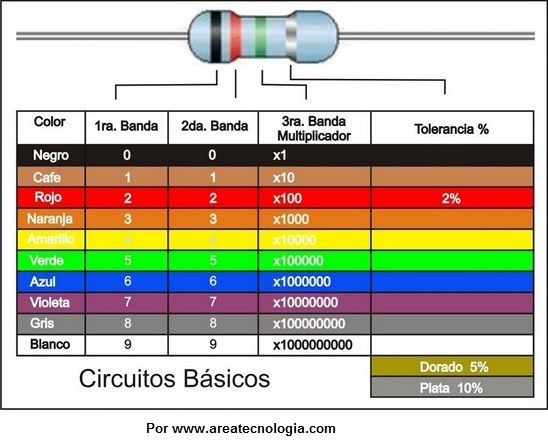
\includegraphics[scale = 0.4]{Imagenes/Fotos/codigo-colores-resistencias.jpg}
\end{center}

\begin{enumerate}
	\item Primer y segundo color: Estos dos colores representan los dígitos significativos del valor nominal del resistor. Cada color está asociado con un número del 0 al 9. Por ejemplo, el color marrón representa el número 1, el color rojo representa el número 2, y así sucesivamente.
	\item Tercer color: Este color indica el multiplicador que se aplica al valor nominal. Cada color tiene un valor multiplicador asociado que va desde $10^0$ (color negro) hasta $10^{9}$ (color blanco). Por ejemplo, el color amarillo indica un multiplicador de x10000, mientras que el color azul indica un multiplicador de x1000000.
	\item Cuarto color (opcional): En algunos resistores, puede haber una cuarta banda de color que indica la tolerancia. El color de esta banda se relaciona con un porcentaje específico de tolerancia. Por ejemplo, el color dorado indica una tolerancia del 5$\%$, mientras que el color plateado indica una tolerancia del 10$\%$.
\end{enumerate}
\section{Descripción de materiales.}

\begin{center}

	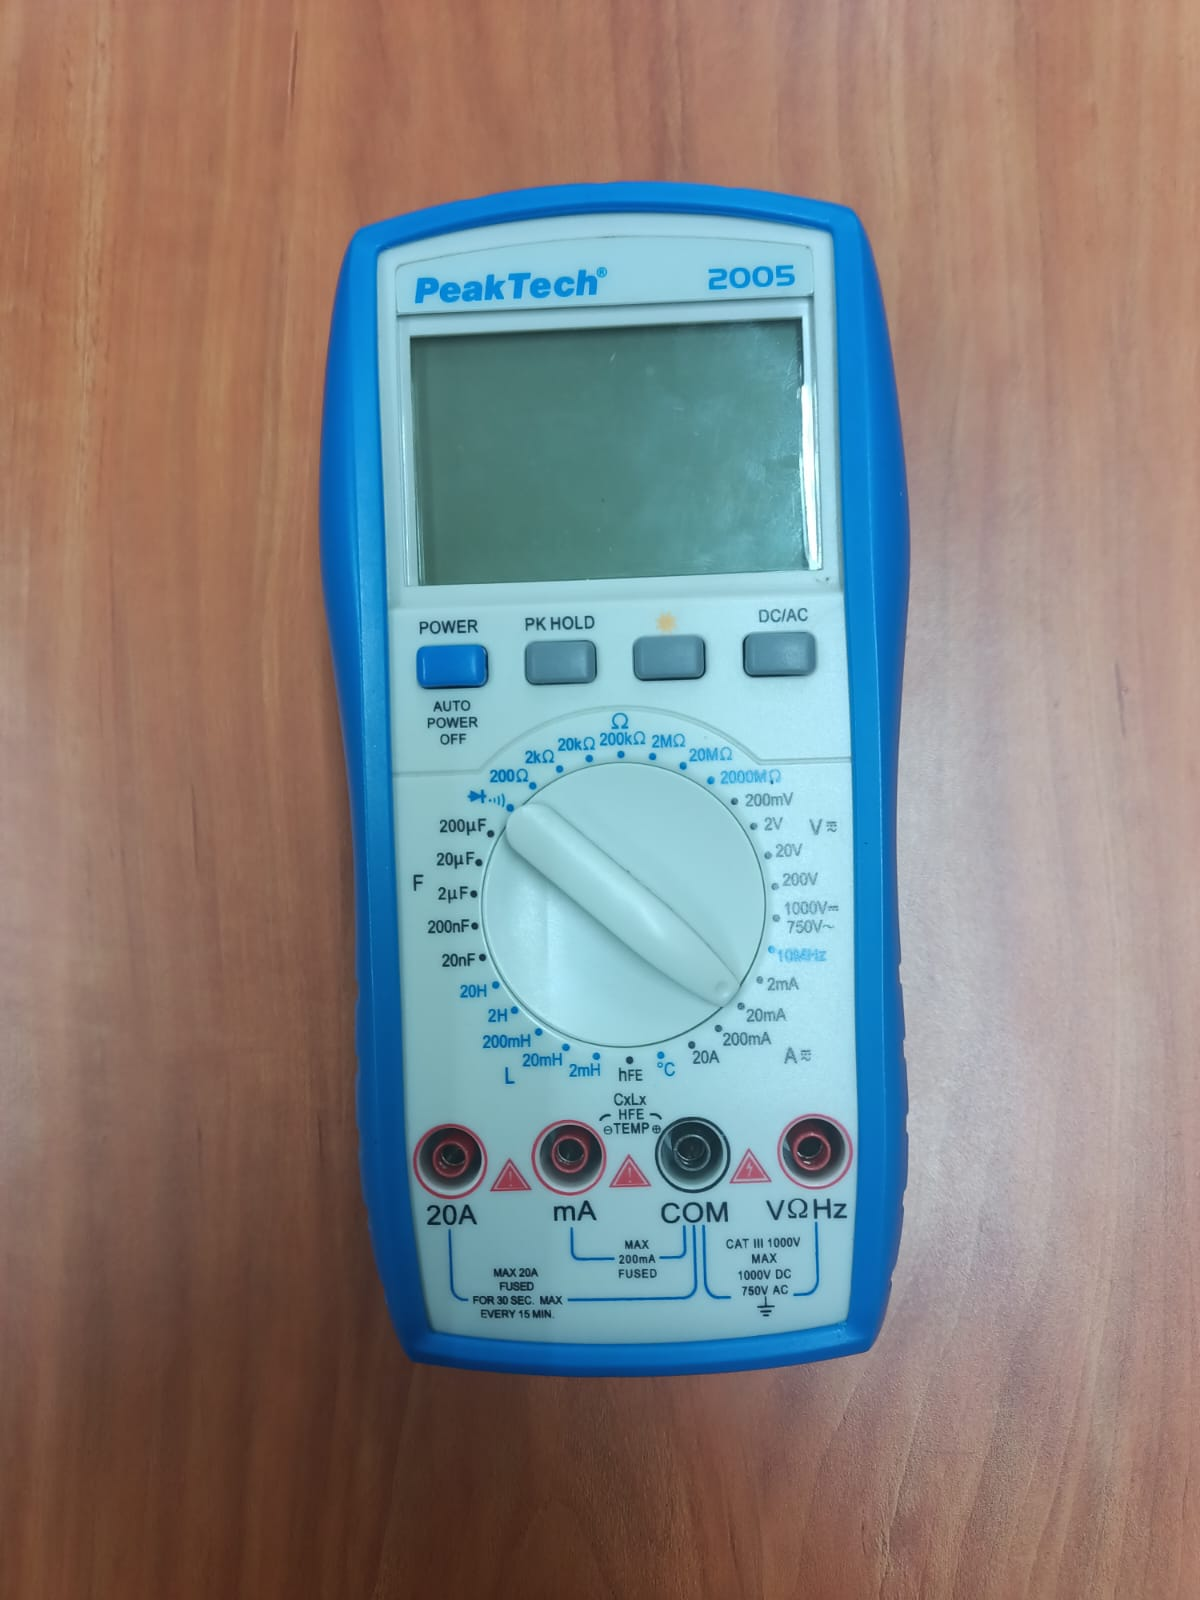
\includegraphics[scale = 0.1]{Imagenes/Material/MultiD.jpeg}\\
	Multímetro Digital.

	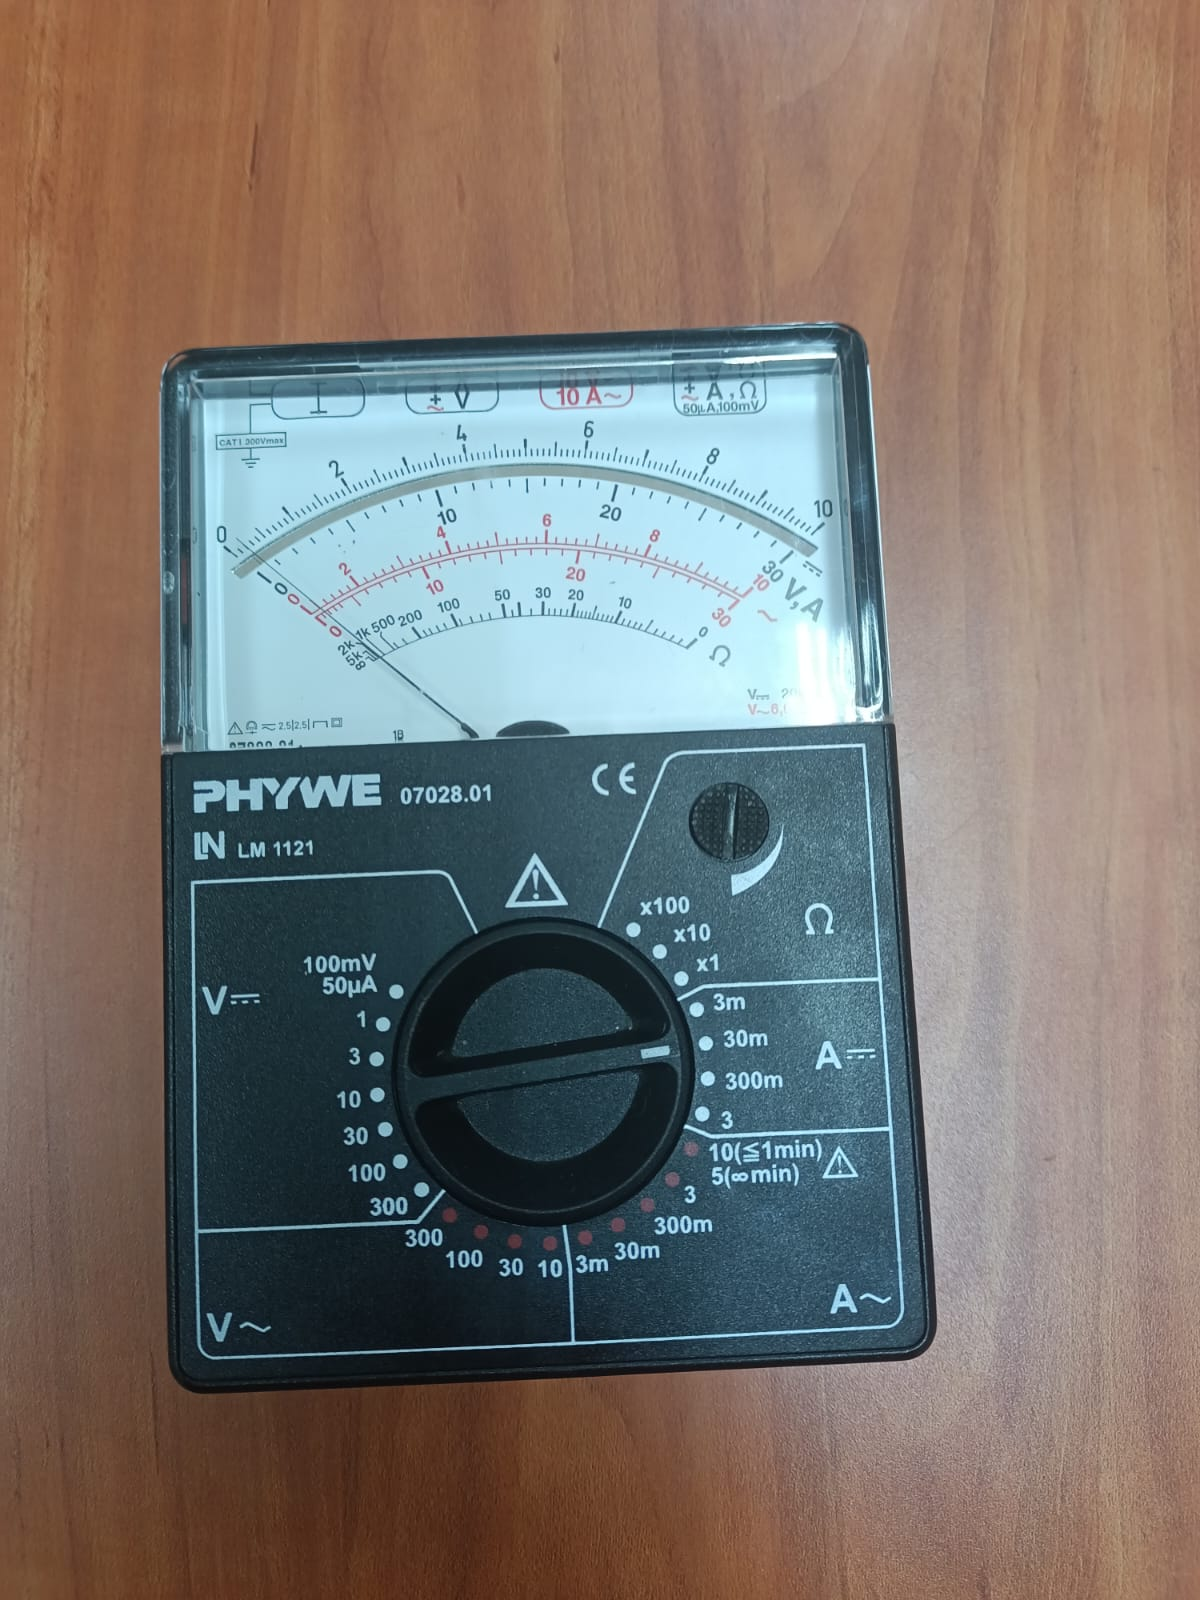
\includegraphics[scale = 0.1]{Imagenes/Material/MultiA.jpeg}\\
	Multímetro Analógico.

	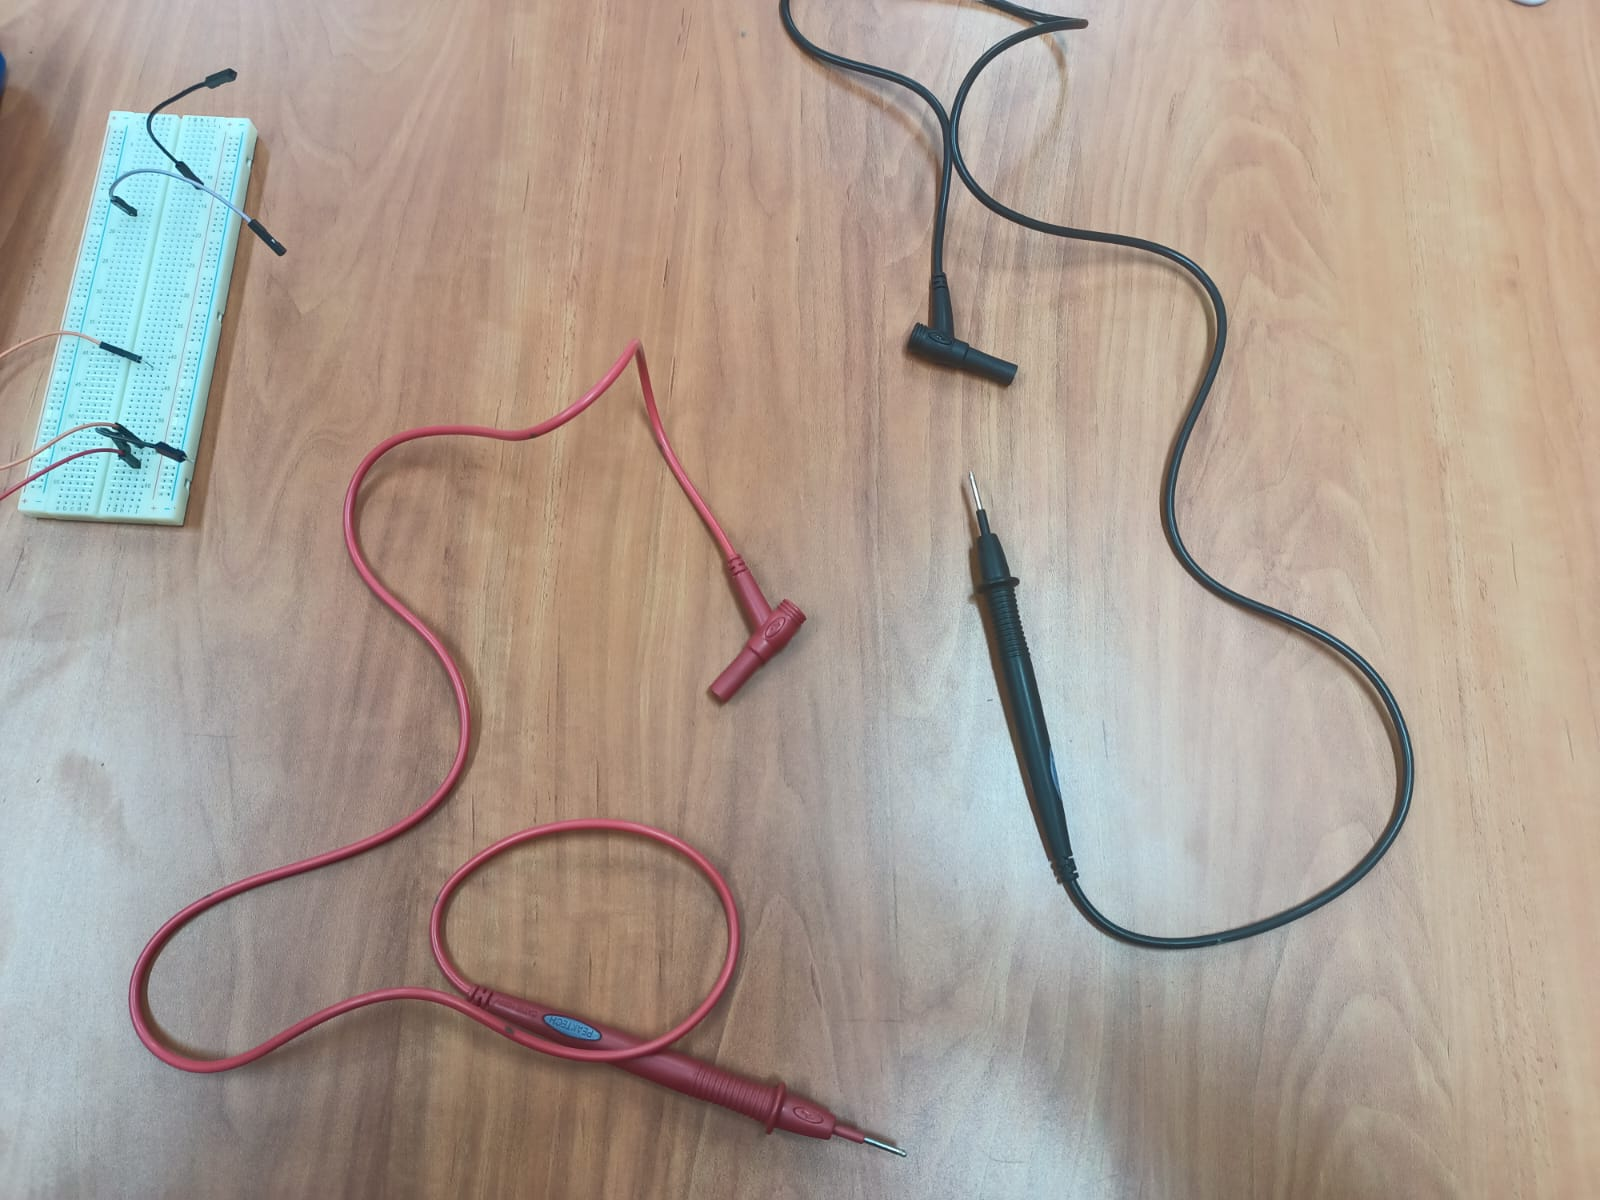
\includegraphics[scale = 0.1]{Imagenes/Material/Puntas.jpeg}\\
	Puntas para multímetro.

	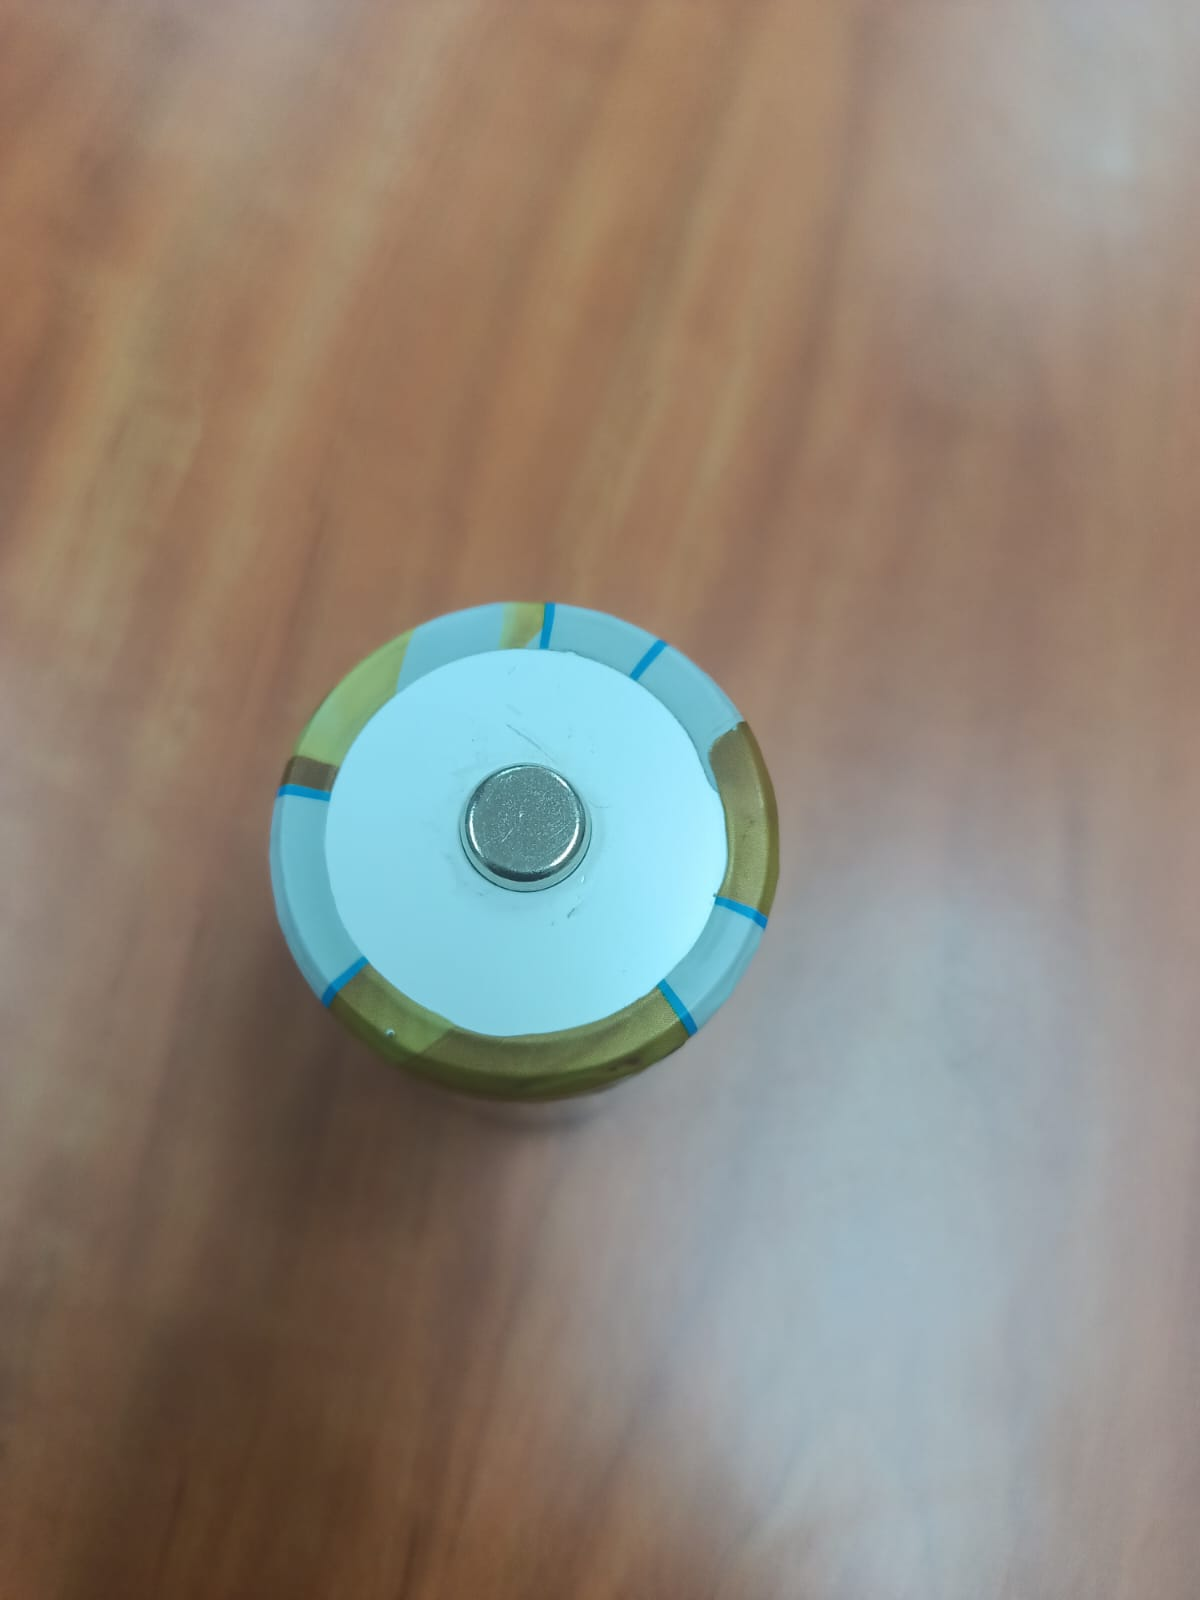
\includegraphics[scale = 0.1]{Imagenes/Material/PilaD.jpeg}\\
	Pila tipo "D" de 1.5 V.

	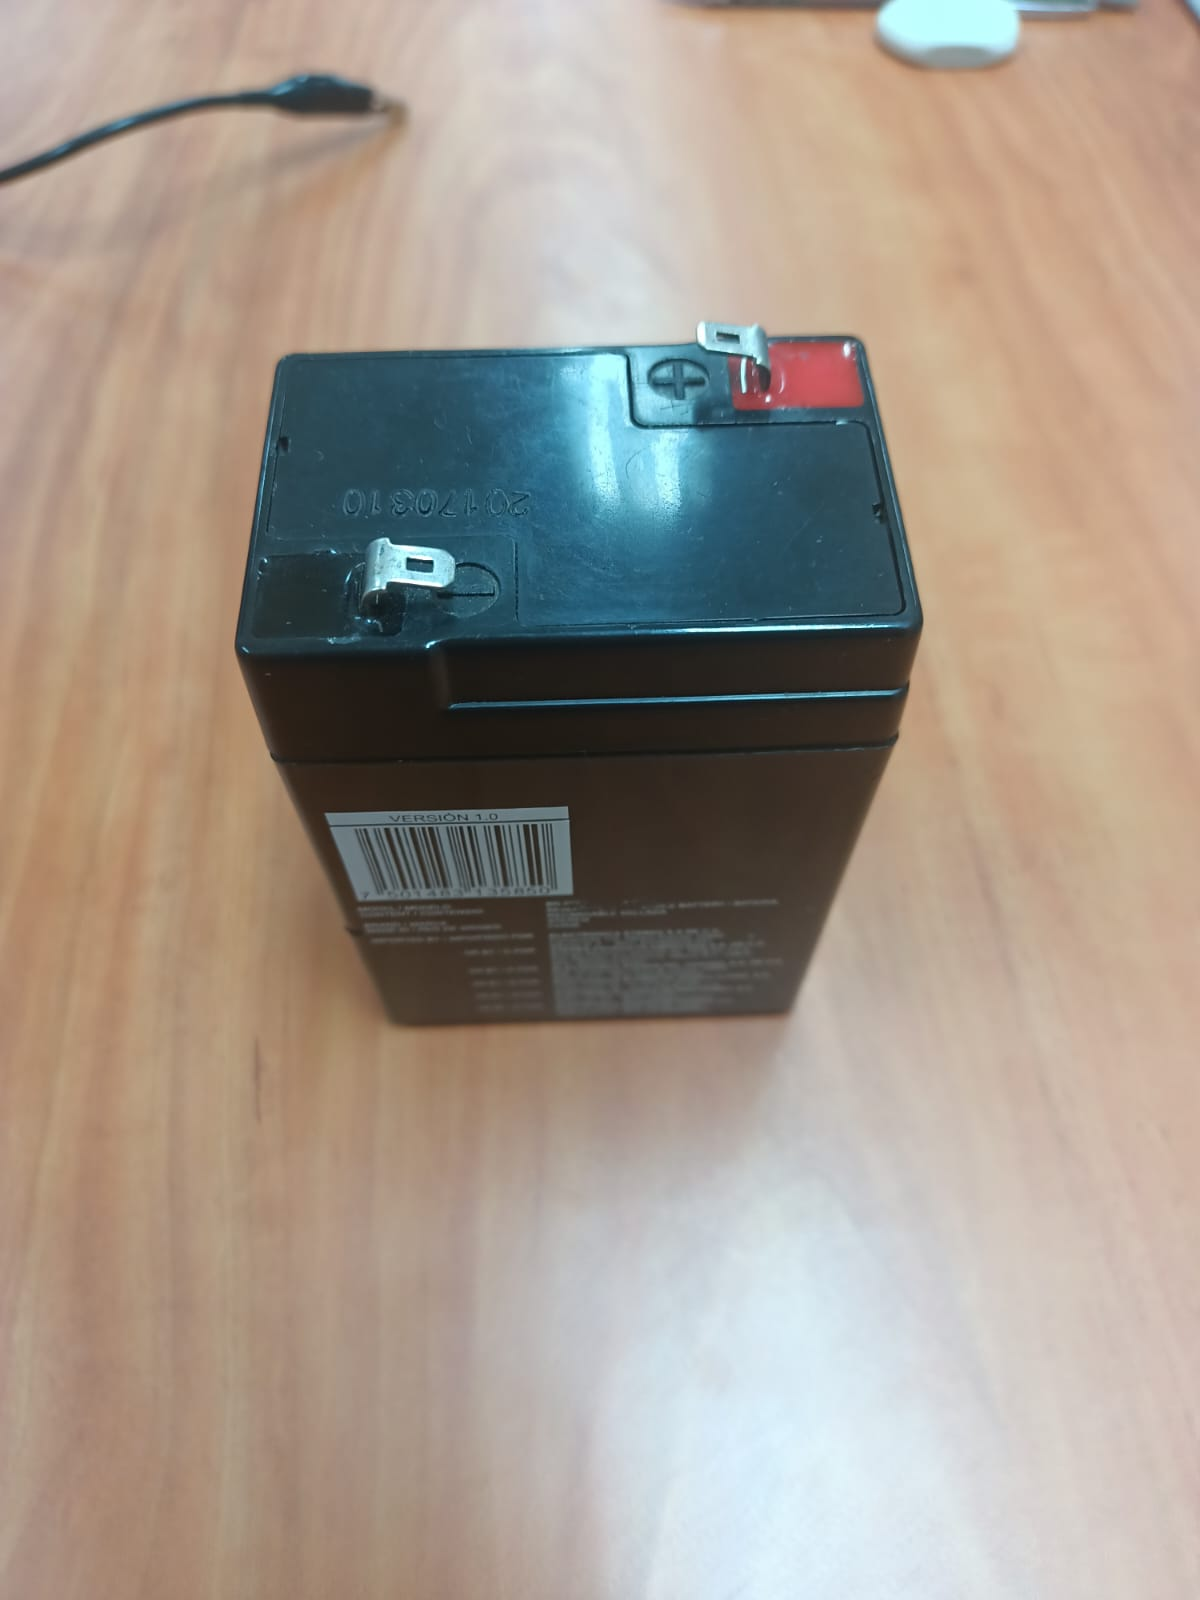
\includegraphics[scale = 0.1]{Imagenes/Material/PilaDes.jpeg}\\
	Pila de valor desconocido.

	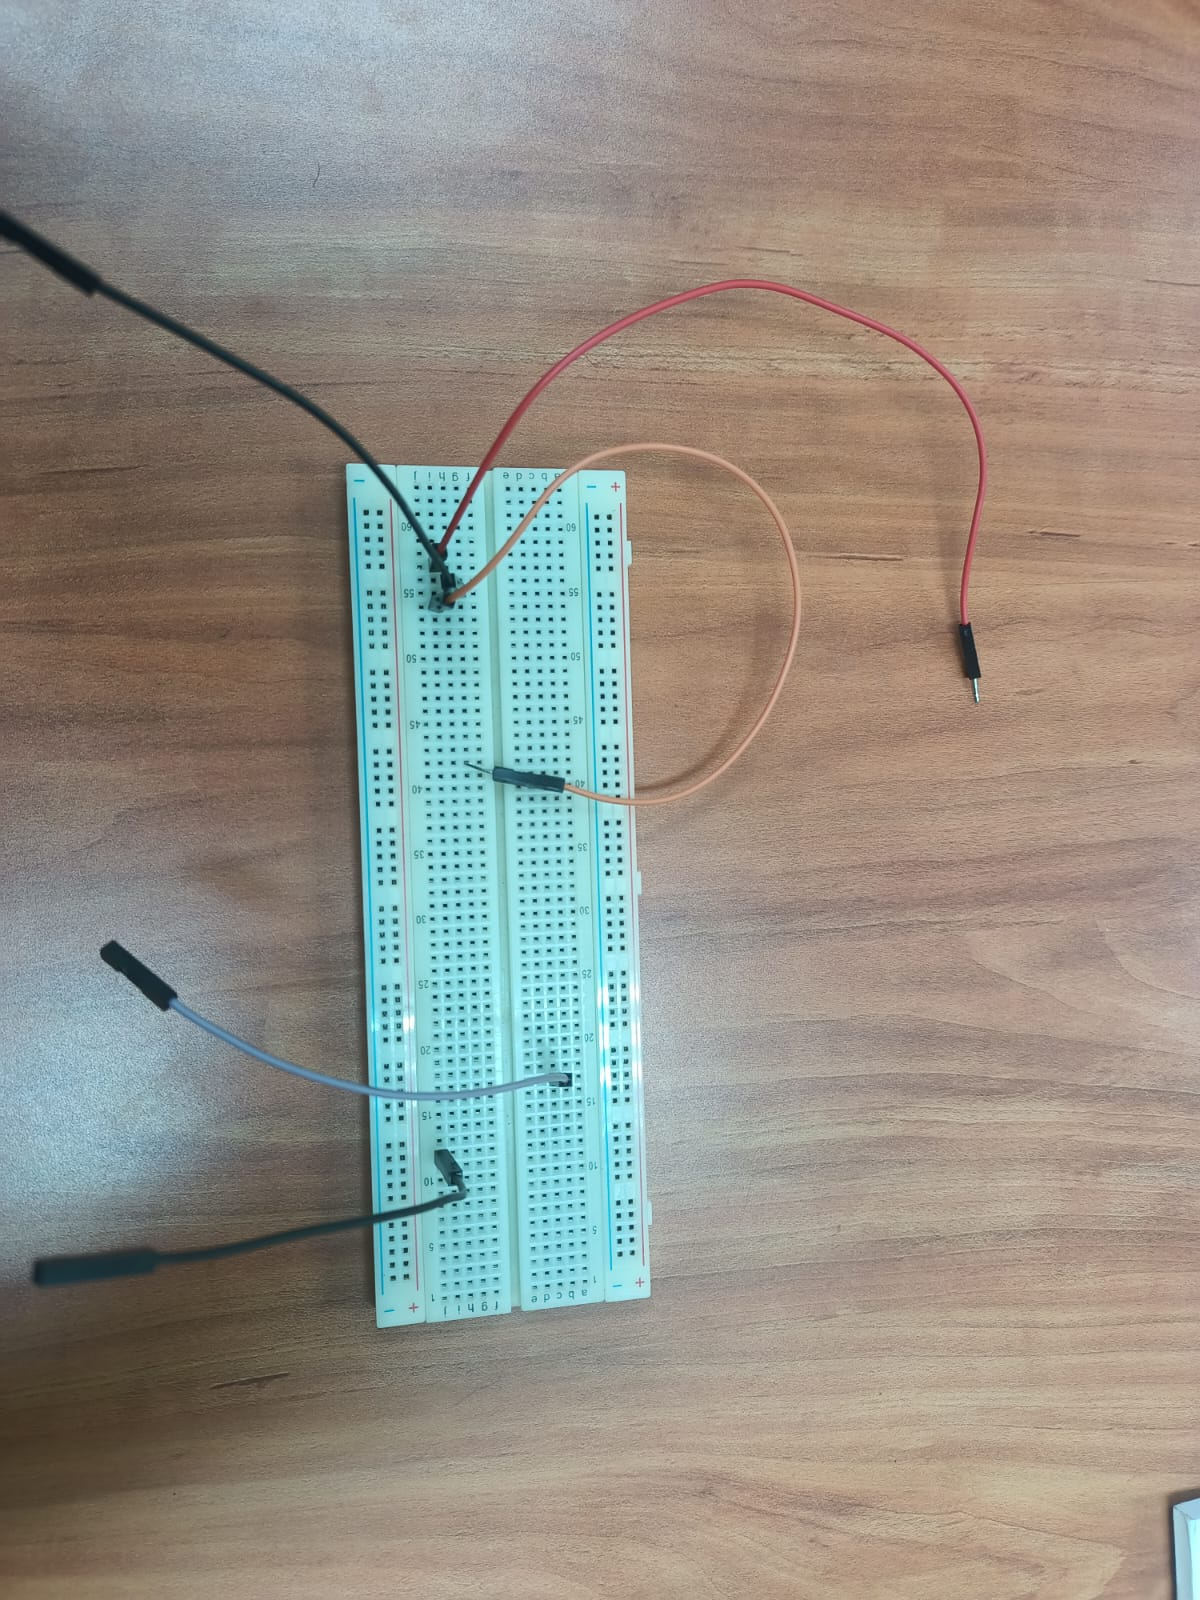
\includegraphics[scale = 0.1]{Imagenes/Material/Protoboard y jumper.jpeg}\\
	Protoboard y Jumpers.

	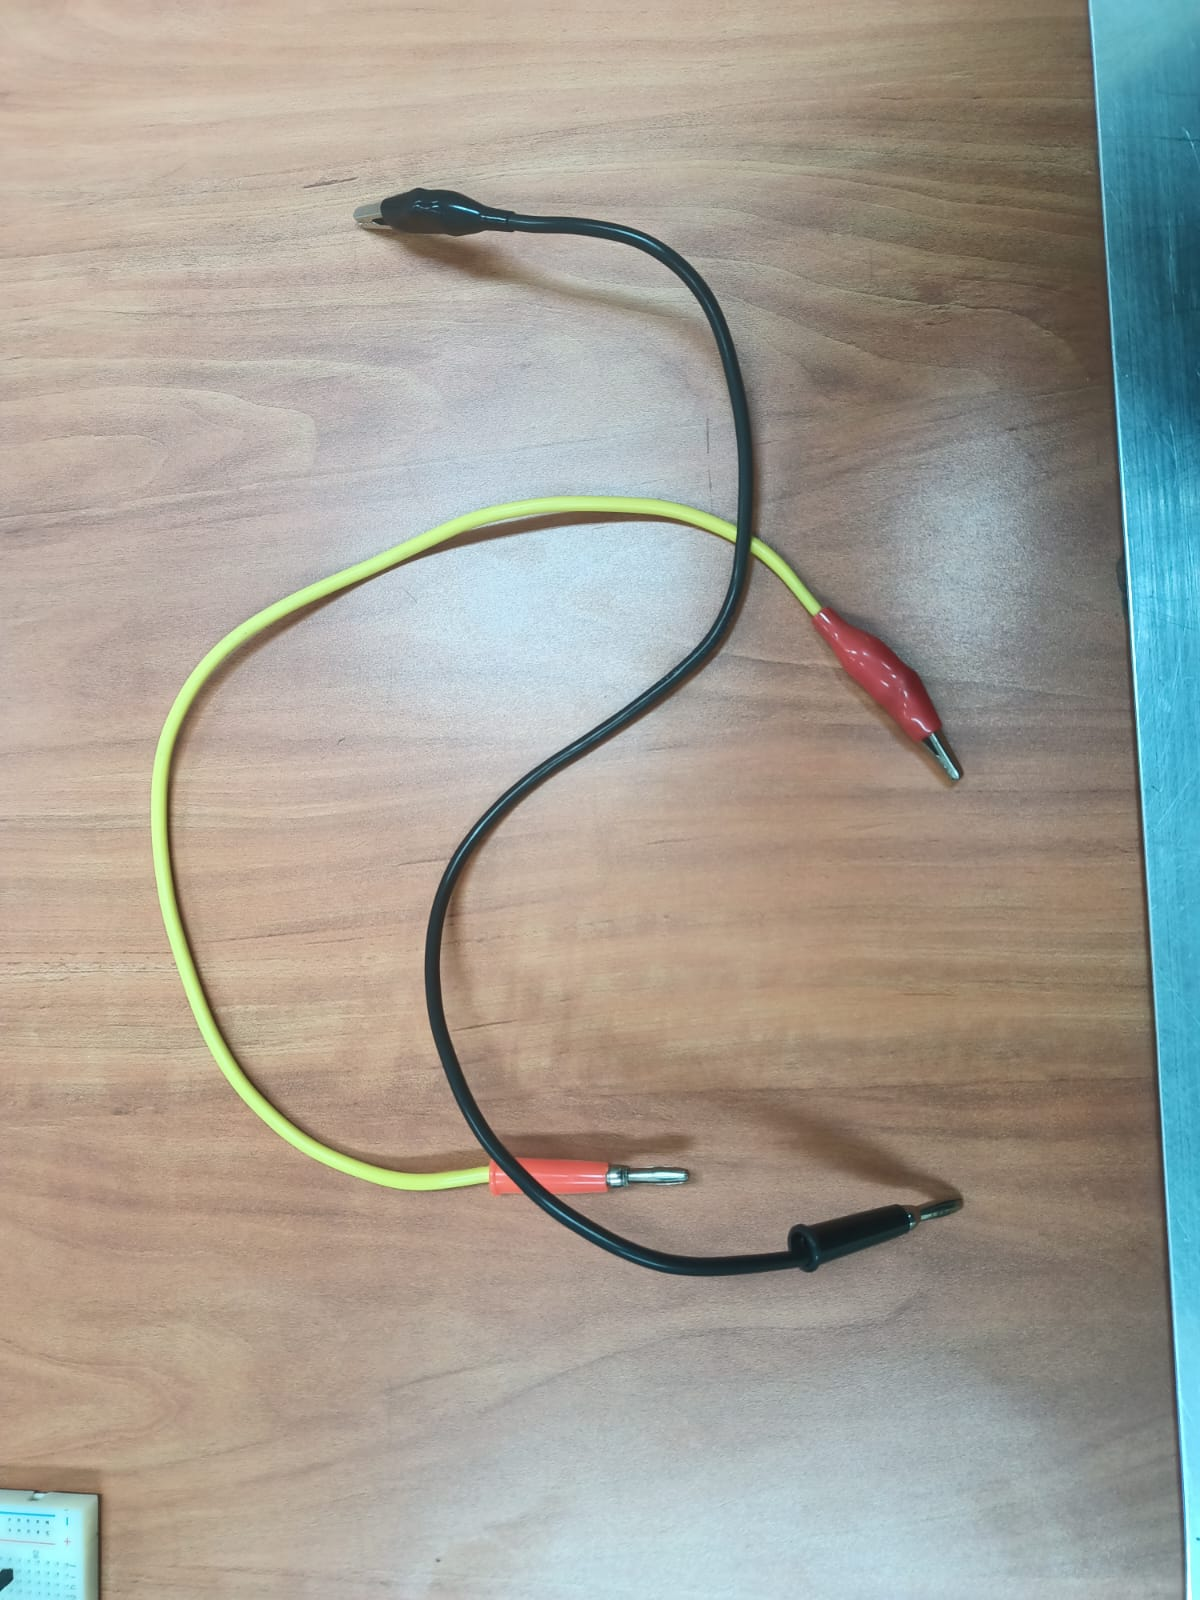
\includegraphics[scale = 0.1]{Imagenes/Material/Caimanban.jpeg}\\
	Cables <<Caimán-Banana>>.

	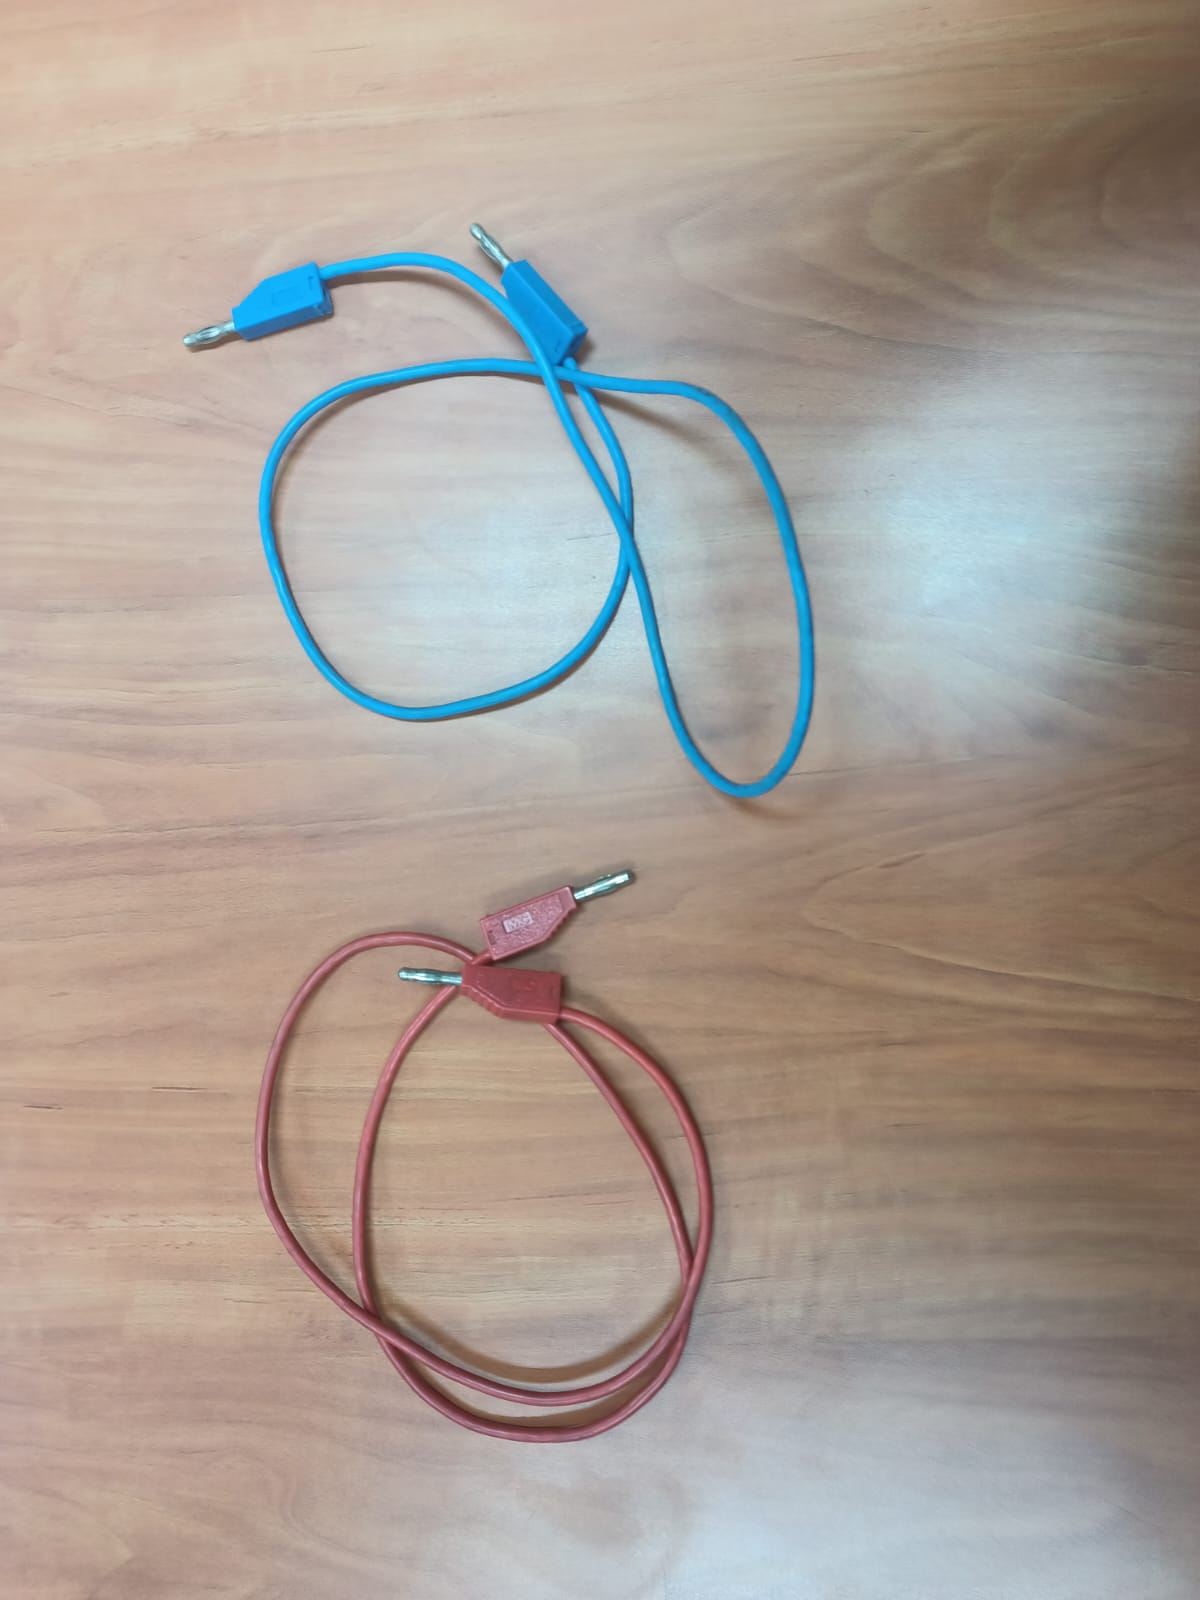
\includegraphics[scale = 0.1]{Imagenes/Material/banban.jpeg}\\
	Cables <<Banana-Banana>>.

	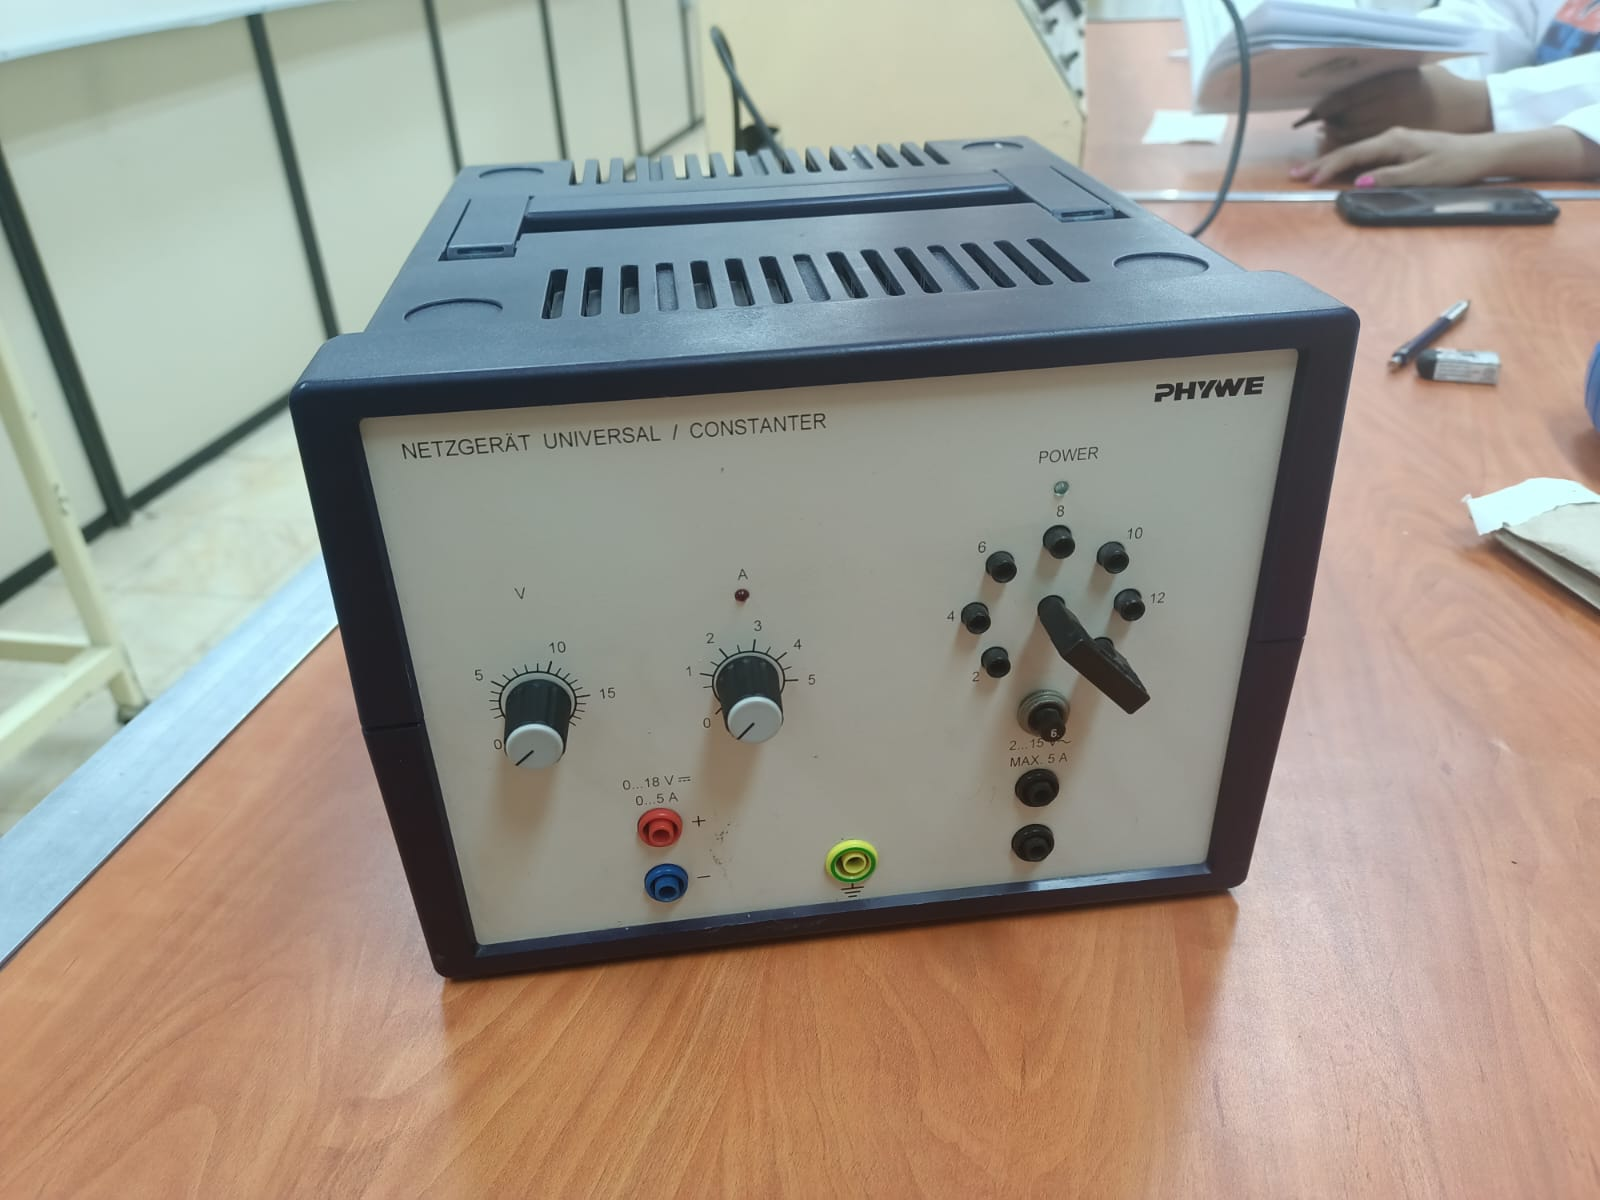
\includegraphics[scale = 0.1]{Imagenes/Material/FuenteVariable.jpeg}\\
	Fuente de alimentación regulada.

	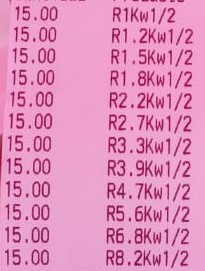
\includegraphics[scale = 1]{Imagenes/Material/Resistencias.jpeg}\\
	Resistencias de valores entre 1K$\Omega$ y 9K$\Omega$

\end{center}


\section{Desarrollo experimental.}

\subsection{Reconocimiento del multímetro.}

Tome el multímetro digital y reconozca lo siguiente:
\begin{enumerate}
	\item La marca y modelo del multímetro.
	\item Como encender el multímetro.
	\item Cuántas posiciones y cuáles son los rangos del multímetro para medir diferencia de potencial eléctricos de Corriente Directa.
	\item Cuántas posiciones y cuáles son los rangos del multímetro para medir corrientes de Corriente Directa y Corriente Alterna.
	\item Cuántos y cuáles son los rangos del multímetro para medir resistencia.
	\item Otras funciones,interruptores y selectores.
\end{enumerate}

\subsection{Mediciones de resistencia(óhmetro).}

\begin{enumerate}
	\item Encienda el multimetro y coloque la perilla en Ohms.
	\item Anote los valores utilizando el código de colores para resistores.
	\item Mida los resistores y anote los valores obtenidos en una tabla.
	\item Compare el valor nominal con el valor medido.
\end{enumerate}

\subsection{Mediciones de continuidad.}

\begin{enumerate}
	\item Utilizando el medidor de continuidad o en la escala de resistencia más baja identifique como está constituida una protoboard.
	\item Elabore un diagrama según lo observado.
\end{enumerate}

\subsection{Mediciones de diferencia de potencial eléctrico(vóltmetro).}

\begin{enumerate}
	\item Coloque la perilla del multímero en volts y ubique correctamente el selector de tipo de corriente en Corriente Directa.
	\item Mida el diferencia de potencial eléctrico de las pilas y anote sus valores.
	\item Utilice la fuente regulada, ubique las salidas de corriente directa y realice tres mediciones diferentes respetando la polaridad.
\end{enumerate}

\subsection{Mediciones de diferencia de potencial eléctrico de corriente alterna(vóltmetro).}

\begin{enumerate}
	\item Ubique un contacto como el mostrado en la siguiente imagen.
	\begin{center}
		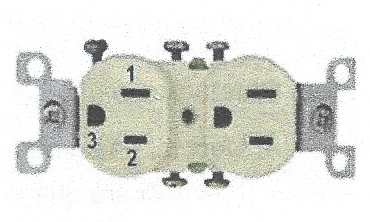
\includegraphics{Imagenes/Fotos/Contacto.png}
	\end{center}
	\item Mida el diferencia de potencial eléctrico entre salidas y anote su valor.
	\item Identifique en el contacto cuál es la fase,el neutro y la tierra física.
\end{enumerate}

\subsection{Mediciones de intensidad de corriente continua(Amperímetro.)}
\begin{enumerate}
	\item Arme el siguiente circuito.
	\begin{center}
		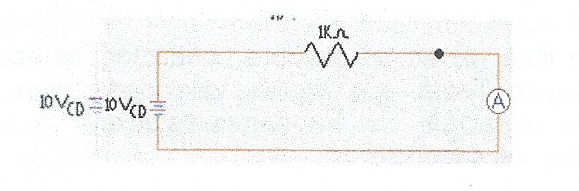
\includegraphics{Imagenes/Fotos/Circuito.png}
	\end{center}
	\item Seleccione una escala de medición adecuada y coloque el selector de Corriente Alterna y Corriente Directa en Corriente Directa.
	\item Mida la corriente en el circuito.
	\item Calcule el valor teórico de la corriente del circuito y compare con el valor medido.
\end{enumerate}

\section{Discusión de materiales.}

\subsection{Diferencias entre multímetro digital y analógico}

Sabemos que los multímetros son básicamente equipos de prueba electrónicos, utilizados con el propósito de determinar varias cantidades como la diferencia de Diferencia de potencial eléctrico, corriente, resistencia, etc. Los multímetros generalmente se clasifican en dos tipos, analógico y digital. La diferencia crucial entre el multímetro analógico y el digital radica en su forma de representar la cantidad que se mide.

\begin{center}

	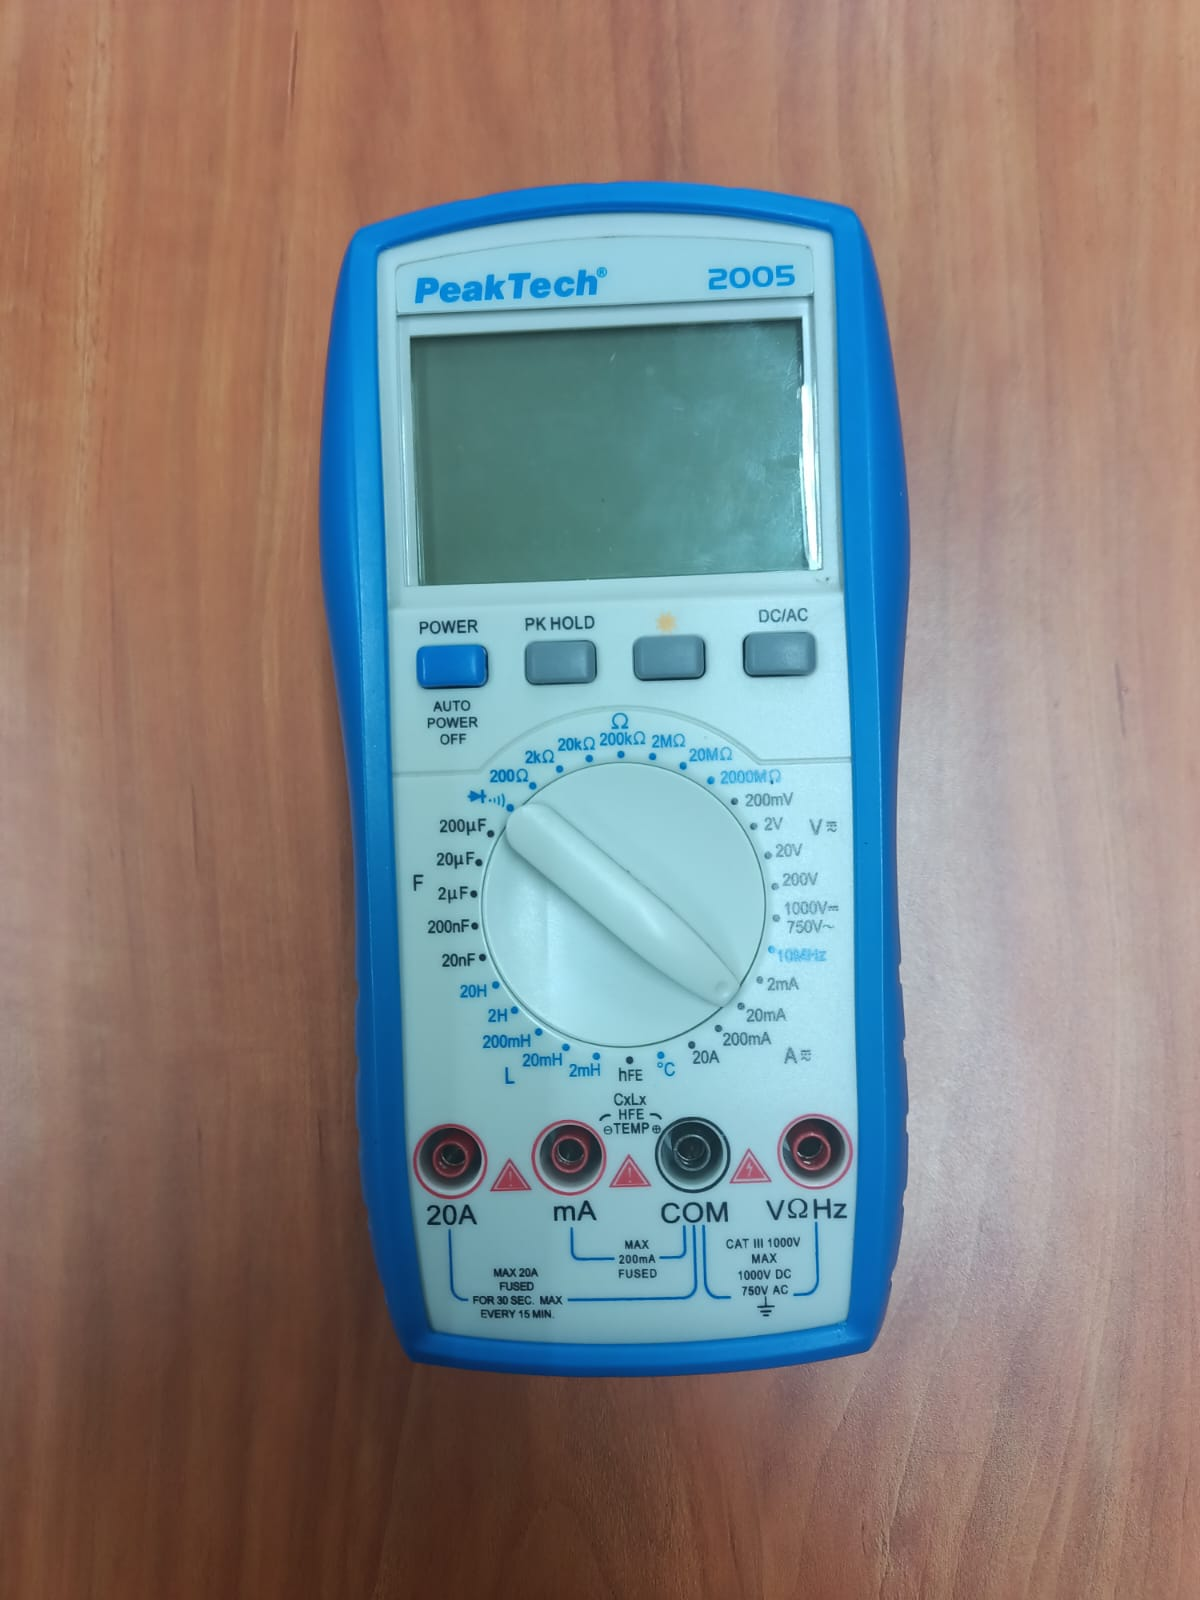
\includegraphics[scale = 0.1]{Imagenes/Material/MultiD.jpeg}\\
	Multimetro Dígital.\\
	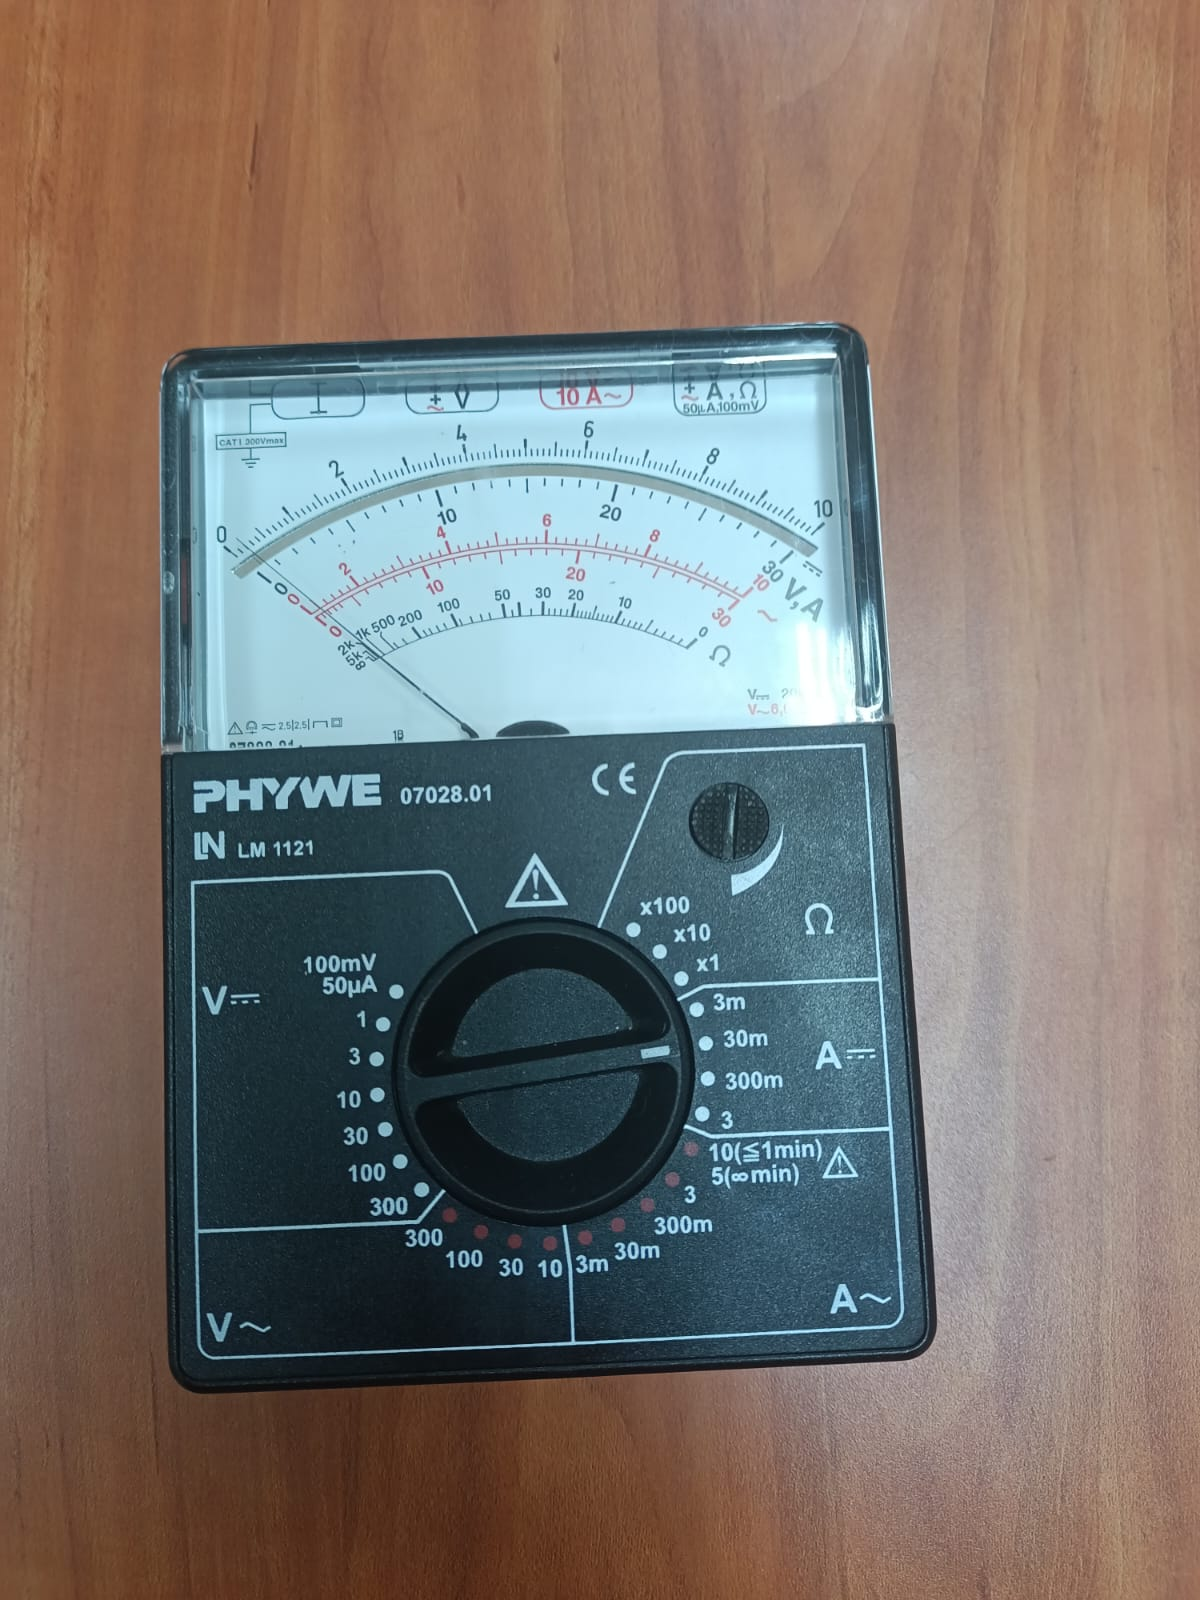
\includegraphics[scale = 0.1]{Imagenes/Material/MultiA.jpeg}\\
	Multímetro Analógico.\\

\end{center}
\begin{enumerate}
\item Un multímetro analógico muestra la cantidad de medición de forma analógica, es decir, mediante la desviación de un puntero en una escala. Por el contrario, un multímetro digital muestra la cantidad en formato digital, es decir, mediante el uso de dígitos.
\item Los multímetros analógicos muestran el resultado en forma analógica, por lo que no requieren un convertidor analógico a digital. Sin embargo, un convertidor digital necesita específicamente un convertidor de analógico a digital en su interior. La exactitud de multímetros analógicos es comparativamente bajo en comparación con el multímetro digital. Como los multímetros digitales generan resultados más precisos que los analógicos.
\item Los multímetros analógicos se utilizan para medir cantidades como diferencia de potencial, corriente y resistencia. Mientras que un multímetro digital junto con estos tres mide la impedancia, la capacitancia, etc. y, a veces, se usa con fines de prueba.
\item Los multímetros analógicos se calibran manualmente, sin embargo, la calibración automática es la ventaja de un multímetro digital.
\item Los multímetros analógicos son bastante difíciles de usar. Mientras que los multímetros digitales brindan facilidad de medición.
\item La presencia de componentes como codificador, ADC, LCD, circuitos lógicos, etc. hace que el circuito de un multímetro digital sea más complejo que el de los multímetros analógicos ya que estos componentes no están presentes en él.
\item Los multímetros analógicos son muy sensibles al recibir golpes.
\item Multímetro analógico muestra menos susceptibilidad al ruido eléctrico durante la medición. Mientras que los multímetros digitales son más susceptibles al ruido eléctrico.
\item La impedancia de entrada de los medidores analógicos es variable, por lo que cambia con el rango. Mientras que es constante en multímetro digital para todos los rangos.
\item La medida máxima permitida frecuencia es bajo para multímetros analógicos mientras que es bastante alto para medidores digitales.
\item Para representar la polaridad inversa, un medidor analógico, el puntero se desvía hacia la izquierda. Mientras que en multímetro digital, la polaridad inversa se indica con un signo negativo.
\end{enumerate}

\subsection{¿Pilas o acumuladores?}

En el habla común, suele darse el nombre de <<Pila>> o <<Batería>> a cualquier elemento que sea una fuente de energía eléctrica obtenida por medio de fenómenos químicos, sin embargo, existe una diferencia fundamental al momento de hablar de este tipo de fuentes y es que las pilas se refieren a aquellos dispositivos que están constituidos por uno o varios elementos primarios que no pueden ser regenerados y por tanto no son recargables, mientras que aquellas fuentes que pueden ser recargables, su nombre correcto es acumuladores.

Con esto, se puede establecer que en la práctica se trabaja con una pila y un acumulador de diferencia de potencial eléctrico desconocido.

\begin{center}
	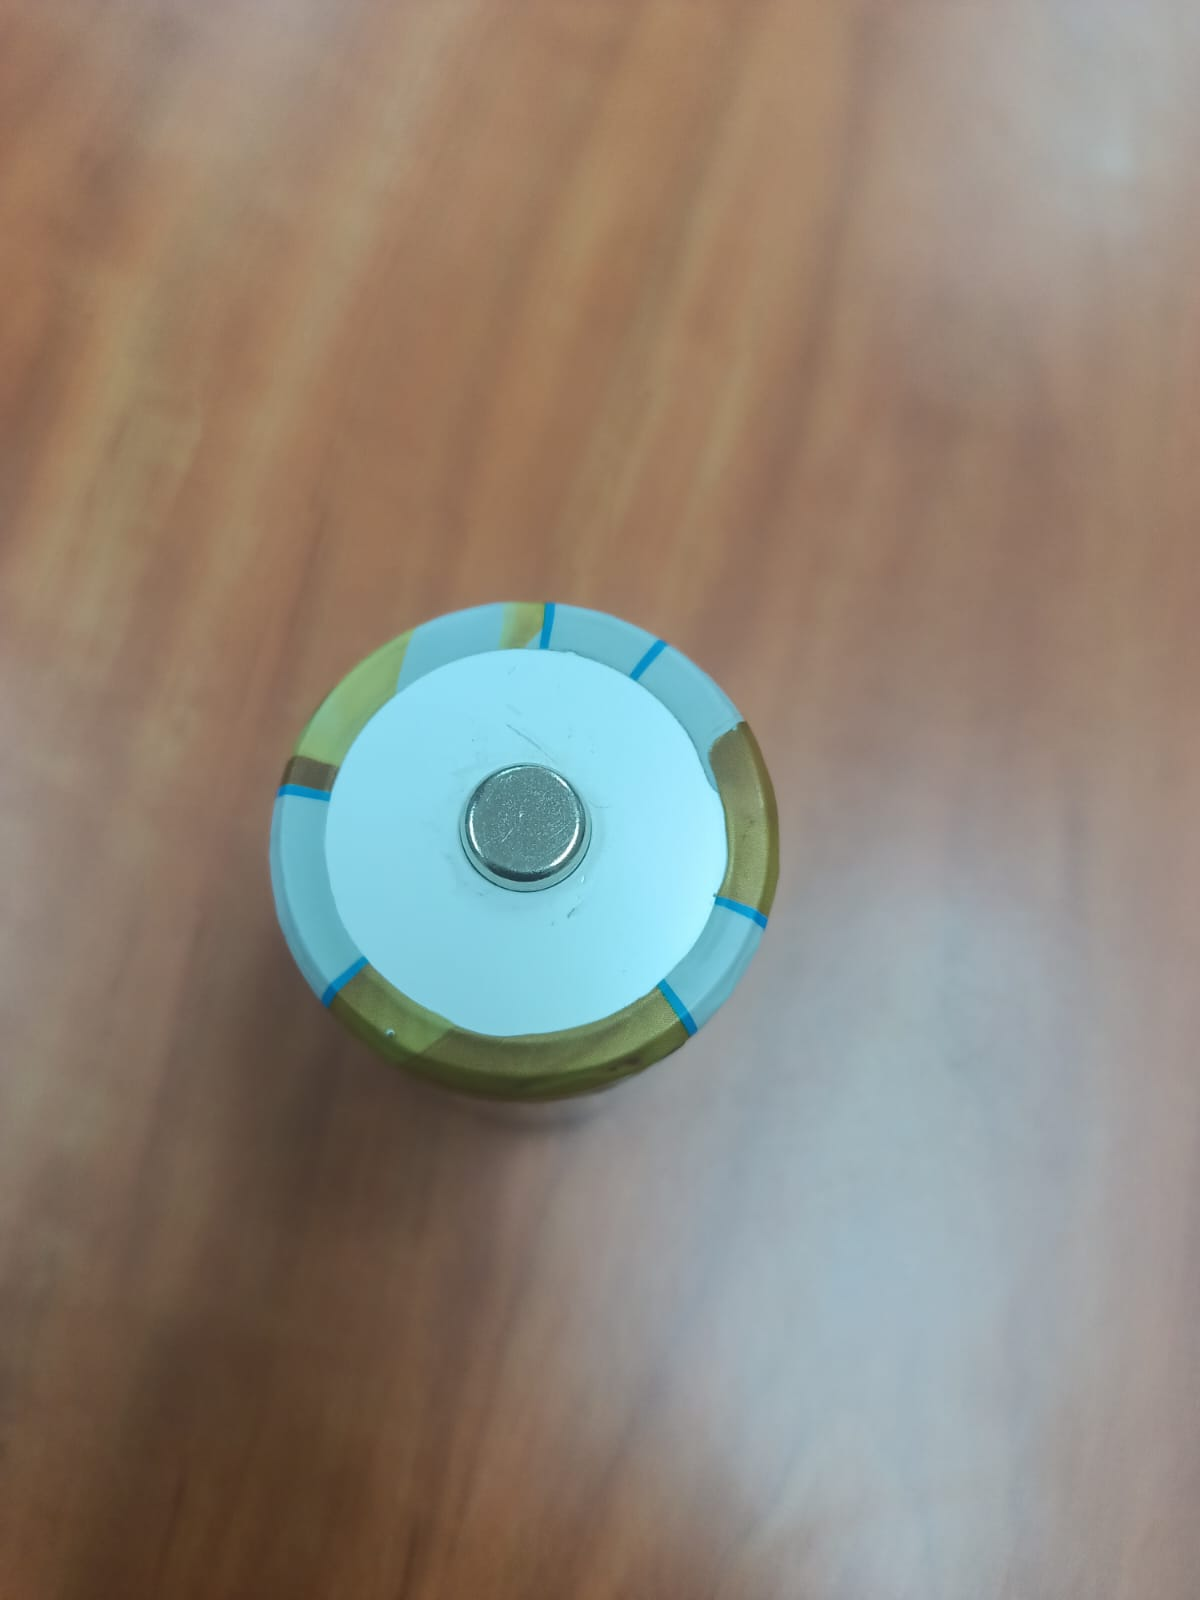
\includegraphics[scale = 0.1]{Imagenes/Material/PilaD.jpeg}\\
	Pila tipo "D".\\
	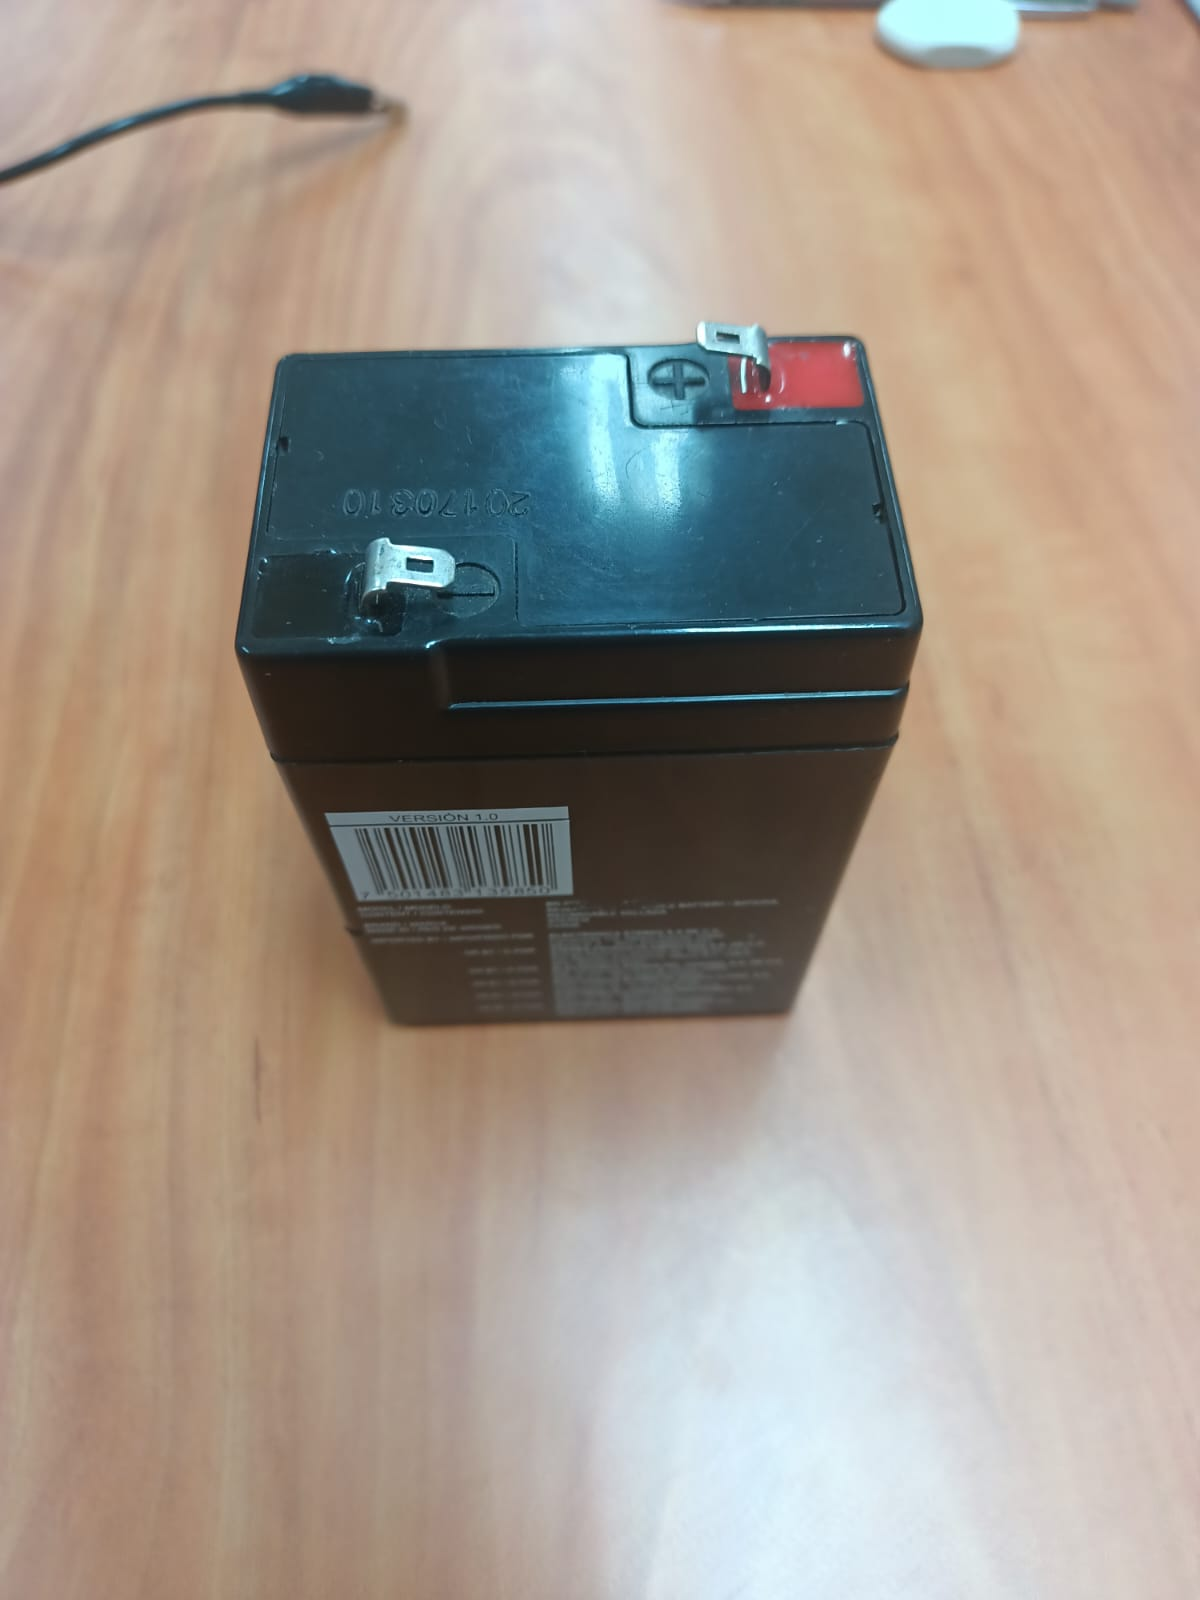
\includegraphics[scale = 0.1]{Imagenes/Material/PilaDes.jpeg}\\
	Acumulador de diferencia de potencial eléctrico desconocido.\\
\end{center}

\subsection{Protoboard}

Una Protoboard es un instrumento que permite probar el diseño de un circuito sin la necesidad de soldar o desoldar componentes. Las conexiones en una Protoboard se hacen con solo insertar los componentes lo que permite armar y modificar circuitos con mayor velocidad.

Las Protoboard tienen tres partes: el canal central, las pistas, y los buses. El canal central, ubicado en la parte media, se conectan los circuitos integrados para mantener aislados los pines de ambos lados del circuito integrado. Los buses se encuentran en los lados de la Protoboard, y generalmente se emplean para conectar la tierra del circuito y su diferencia de potencial eléctricos de alimentación.El resto de los orificios de la Protoboard pertenecen a las pistas, las cuales están separadas por filas y columnas. Las filas están indicadas con números y las columnas están indicadas con letras.

\begin{center}
	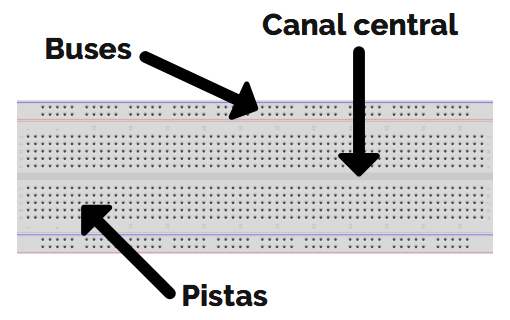
\includegraphics[scale = 0.5]{Imagenes/Fotos/Estructura-protoboard.png}\\
	Partes de la protoboard.\\
	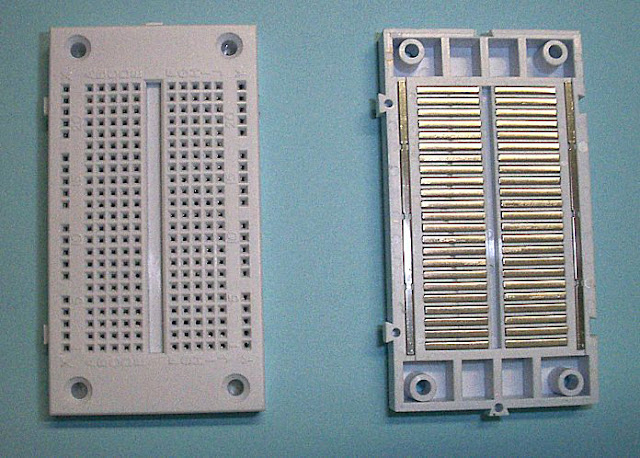
\includegraphics[scale = 0.3]{Imagenes/Fotos/ProtoboardInterno.jpg}\\
	Estructura interna de la protoboard.\\
\end{center}

Las Protoboard presentan algunas ventajas y desventajas. Entre sus principales ventajas esta que pueden utilizarse tantas veces como se requiera y que son de fácil manejo. Por otra parte, entre sus desventajas esta el inconveniente de que en ocasiones puede haber falsos contactos, los cables empleados pueden tener mala conductividad o estar rotos, lo que hace que las conexiones no sean tan seguras como las de las pistas de un circuito impreso. Otra característica que hay que tomar en cuenta es que las Protoboards no estan diseñadas para trabajar con componentes de gran potencia.
La corriente con la que puede operar una Protoboard varía entre 3 y 5 A según el fabricante.

\subsection{Variación en el valor nominal de los resistores.}

Los valores nominales de los resistores en operación están generalmente basados a 25 °C (temperatura ambiente) por lo que una variación de la temperatura puede ser causante de una variación, otras razones por las cuales la resistencia real de un resistor varía son las siguientes:
\begin{enumerate}
	\item Tolerancia: Los resistores tienen una tolerancia, que es una medida de la variación permisible en su valor nominal. La tolerancia se expresa como un porcentaje y indica cuánto puede desviarse el valor real del resistor con respecto a su valor nominal. Por ejemplo, si tienes un resistor con un valor nominal de 100 $\Omega$ y una tolerancia del 5$\%$, el valor real del resistor puede variar en ±5 $\Omega$, lo que significa que su valor puede estar entre 95 $\Omega$ y 105 $\Omega$.
	\item Fabricación: Durante el proceso de fabricación, pueden ocurrir pequeñas variaciones en las propiedades físicas de los materiales utilizados para construir los resistores. Estas variaciones pueden afectar el valor final del resistor. Además, los métodos de fabricación utilizados, como el tipo de material resistivo, el tamaño y la forma del resistor, pueden influir en su valor nominal.
	\item Desgaste: Con el tiempo, los resistores pueden experimentar desgaste debido a factores como el calor, la humedad y la deformación. Estas condiciones pueden afectar las características eléctricas de los resistores, lo que resulta en cambios en su valor nominal.
\end{enumerate}


\section{Análisis y resultados.}

\subsection{Reconocimiento del multímetro.}
 

\subsubsection{Multímetro Digital Peaktech 2005.}

El multímetro utilizado en la práctica es de marca Peaktech modelo 2005, en el manual de usuario se pueden encontrar todas las funciones con las que cuenta, que se enumeran a continuación.

\begin{enumerate}
	\item Diferencia de Diferencia de potencial eléctrico en corriente directa con un rango de 200mV a 1000V y corriente alterna con un rango de 100mV a 750V
	\item Corriente eléctrica en corriente alterna y corriente directa , ambas con un rango de 2mA hasta 20A con 5 fusibles en cada entrada de A.
	\item Resistencia con un rango de 200 $\Omega$ a 2000M$\Omega$.
	\item Frecuencia con un rango de 2kHz hasta 10 MHz.
	\item Capacitancia con un rango de 20nF hasta 200$\mu$F.
	\item Inductividad con un rango de 2mH hasta 20H.
	\item Temperatura con un rango de -20°C a 1000°C.
	\item Diodo con un rango de 2V.
	\item Prueba de continuidad.
	\item Transistor (hFe).
\end{enumerate}

A continuación se muestran todos los botones con los que cuenta el multímetro. 

\begin{center}
	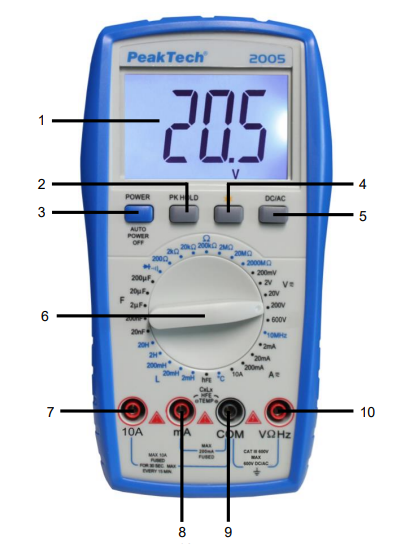
\includegraphics[scale = 0.5]{Imagenes/Marco/Multimetro.PNG}\\
	\begin{enumerate}
		\item Pantalla LCD
		\item Tecla PK Hold. Permite congelar la lectura máxima en pantalla.
		\item Tecla de encendido y apagado. 
		\item Tecla de retroiluminación. Ayuda a tener mejor observación cuando hay poca luz.
		\item Tecla Corriente Directa / Corriente Alterna.
		\item Selector.
		\item Conector de entrada 10 A.
		\item Conector de entrada mA/temp.
		\item Conector de entrada COM.
		\item Conector de entrada V/$\Omega$/Hz.
	\end{enumerate}
\end{center}


\subsection{Mediciones de resistencia(óhmetro).}
\begin{center}
	\begin{adjustbox}{width=245pt}
		\begin{tabular}{|c|c|c|c|c|}
			\hline
			Resistencia & Colores & Tolerancia & Valor nominal (ohms) & Valor medido (ohms) \\
			\hline
			1 & Café, verde, rojo, dorado & $\pm$ 5\% & 1.5k & 1.46k \\
			\hline
			2 & Rojo, azul, rojo, dorado & $\pm$ 5\% & 2.6k & 2.18k \\
			\hline
			3 & Naranja, naranja, naranja, dorado & $\pm$ 5\% & 33k & 32.8k \\
			\hline
			4 & Amarillo, violeta, rojo, dorado & $\pm$ 5\% & 4.7k & 4.75k \\
			\hline
			5 & Azul, verde, rojo, dorado & $\pm$ 5\% & 6.5k & 6.66k \\
			\hline
		\end{tabular}
	\end{adjustbox}
\end{center}

Al medir resistores, no importa con qué polaridad se coloquen las puntas para medirlos, ya que estos no tienen polaridad. Por otro lado, si el multímetro no es automático, es necesario calibrarlo correctamente para obtener una buena medición. Además, se puede utilizar el código de colores que los resistores incluyen para facilitar la identificación y medición precisa.

El resistor con mayor distancia entre su valor nominal y su valor real es el número 2, el cual supera el $\pm$5\% de toleracia que indica su franja dorada, es probable que este resistor tuvo un problema en su fabricación o fue dañado en su transporte. Los demás se encuentran dentro de sus límites permisibles.
\subsection{Mediciones de continuidad.}

\begin{center}
	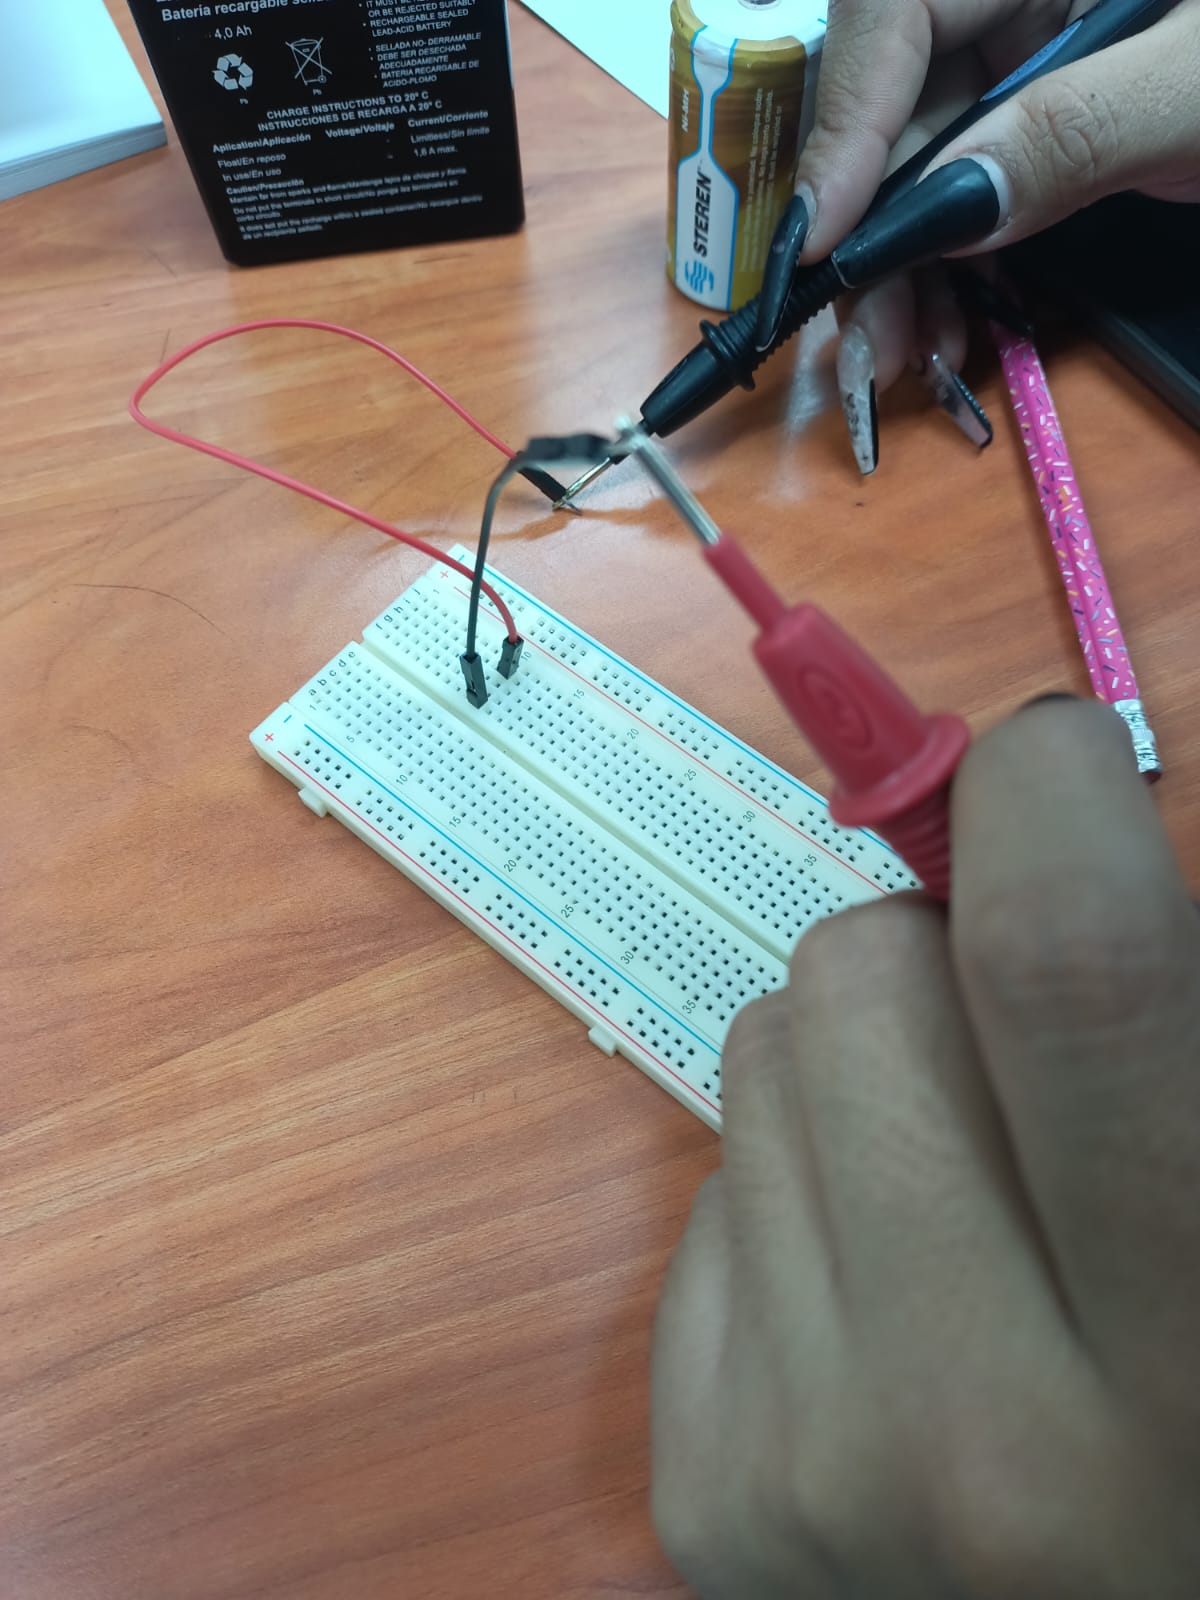
\includegraphics[scale = 0.1]{Imagenes/Fotos/ConFilas.jpeg}\\
	Continuidad en las filas en las pistas.
	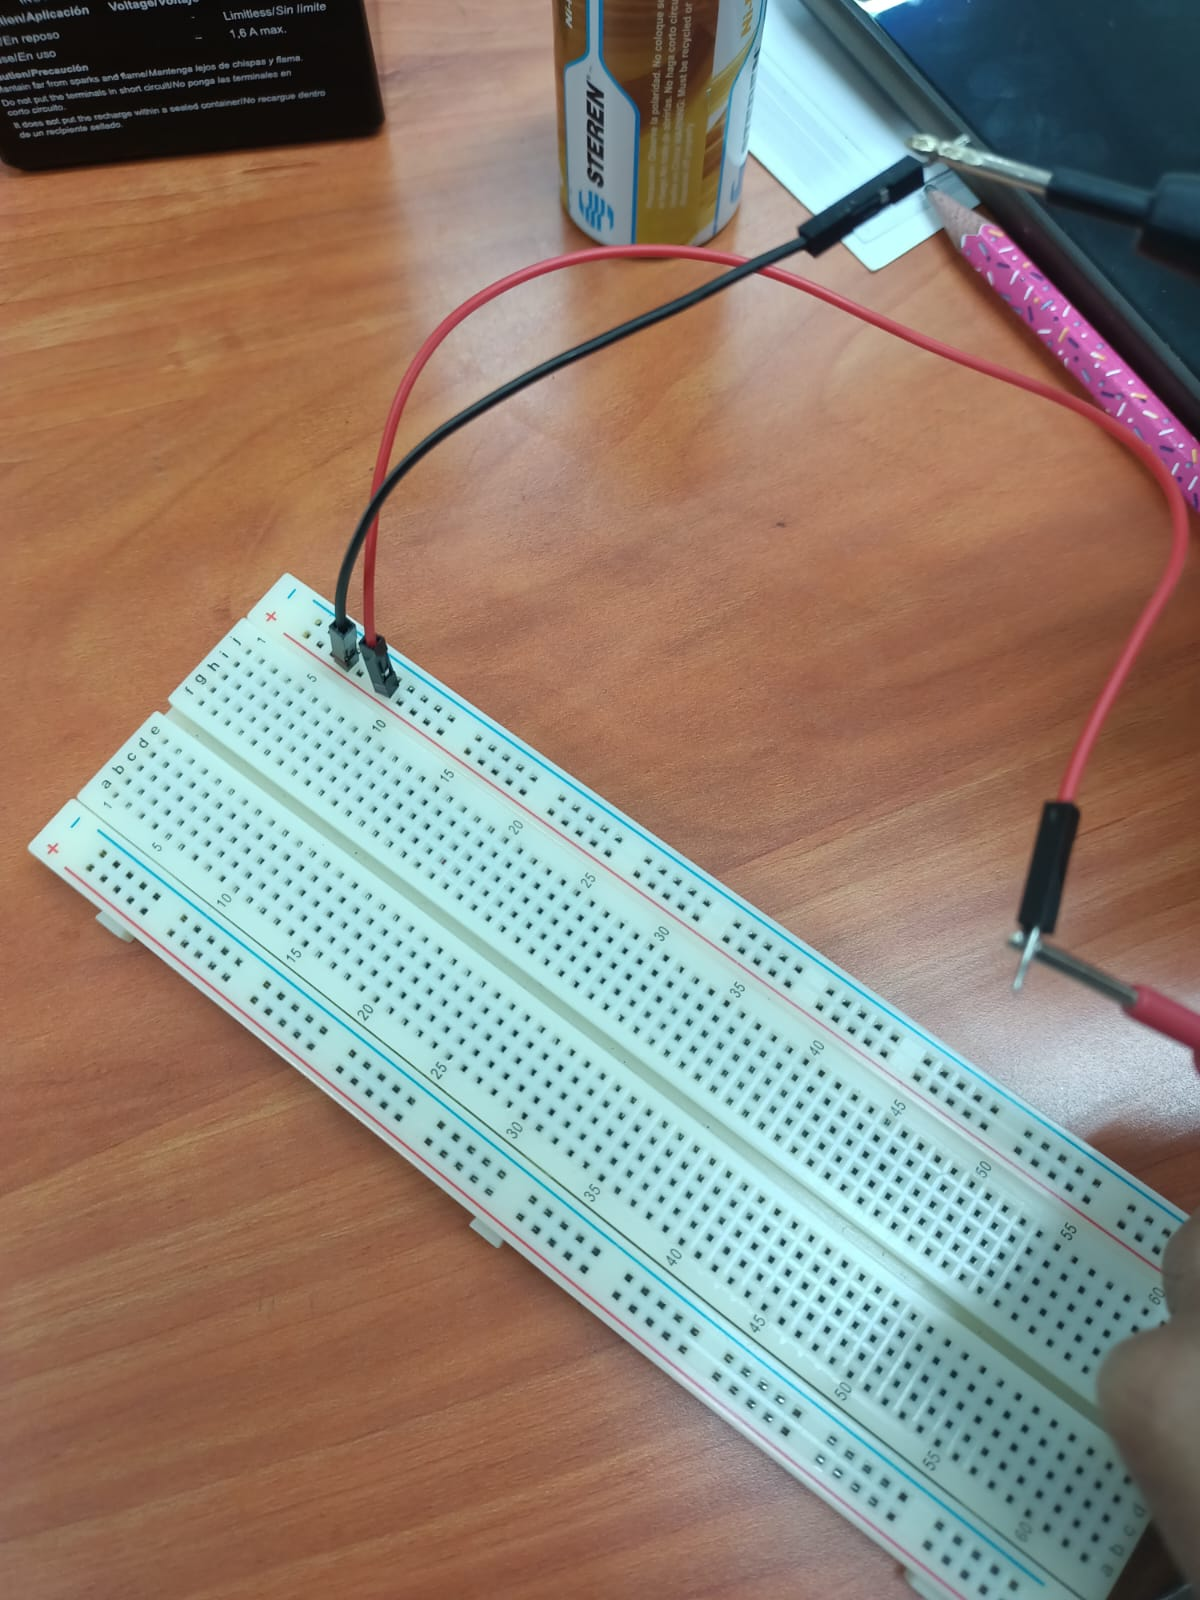
\includegraphics[scale = 0.1]{Imagenes/Fotos/ConColumnas.jpeg}\\
	Continuidad en las columnas en los buses.\\
	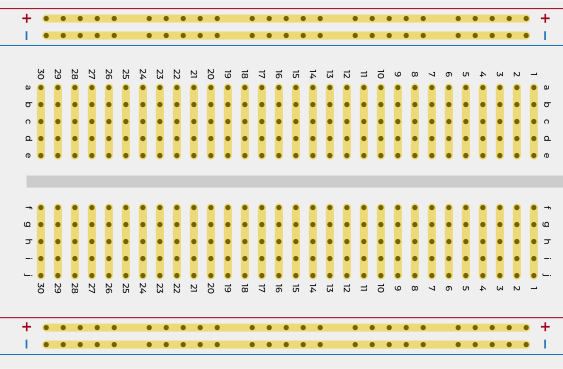
\includegraphics[scale = 0.4]{Imagenes/Fotos/Diagrama.png}\\
	Diagrama de conexiones en la protoboard,se pueden hacer puentes entre pistas y buses para llevar la corriente eléctrica según se necesite.
\end{center}

\subsection{Mediciones de diferencia de potencial eléctrico(vóltmetro).}

Medida de diferencia de potencial eléctrico de la pila y el acumulador.

\begin{tabular}{ p{4cm} p{3cm} }
	\hline
	Pila : & 0.82 volts \\
	\hline
	Acumulador : & 5.9 volts \\
	\hline
\end{tabular}

Según la información que se muestra en la pila , esta debe tener un valor de 1.5 V si está cargada completamente, sin embargo, presenta una diferencia de potencial de 0.82V.

\begin{center}
	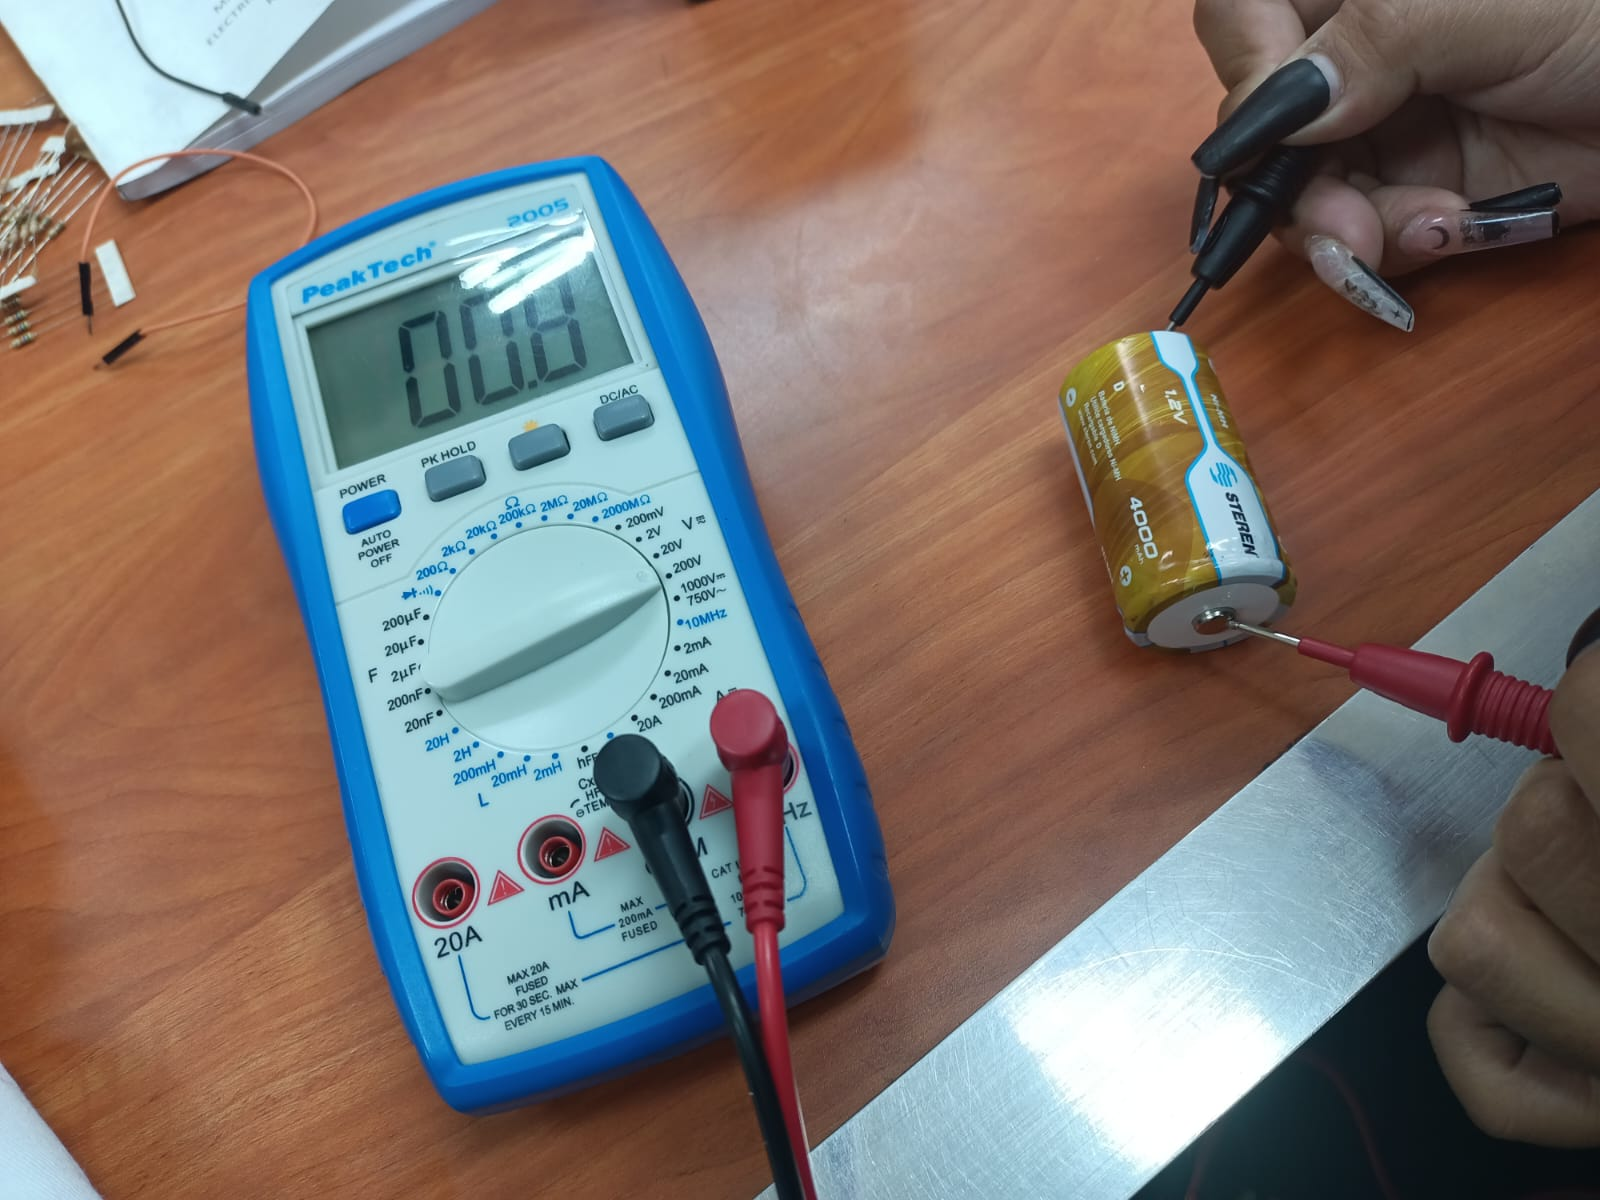
\includegraphics[scale = 0.1]{Imagenes/Fotos/Pila.jpeg}\\
	La imagen muestra un valor de 00.8, es un ejemplo de lo que sucede cuando no se fija bien el rango necesario.
\end{center}

\begin{center}
	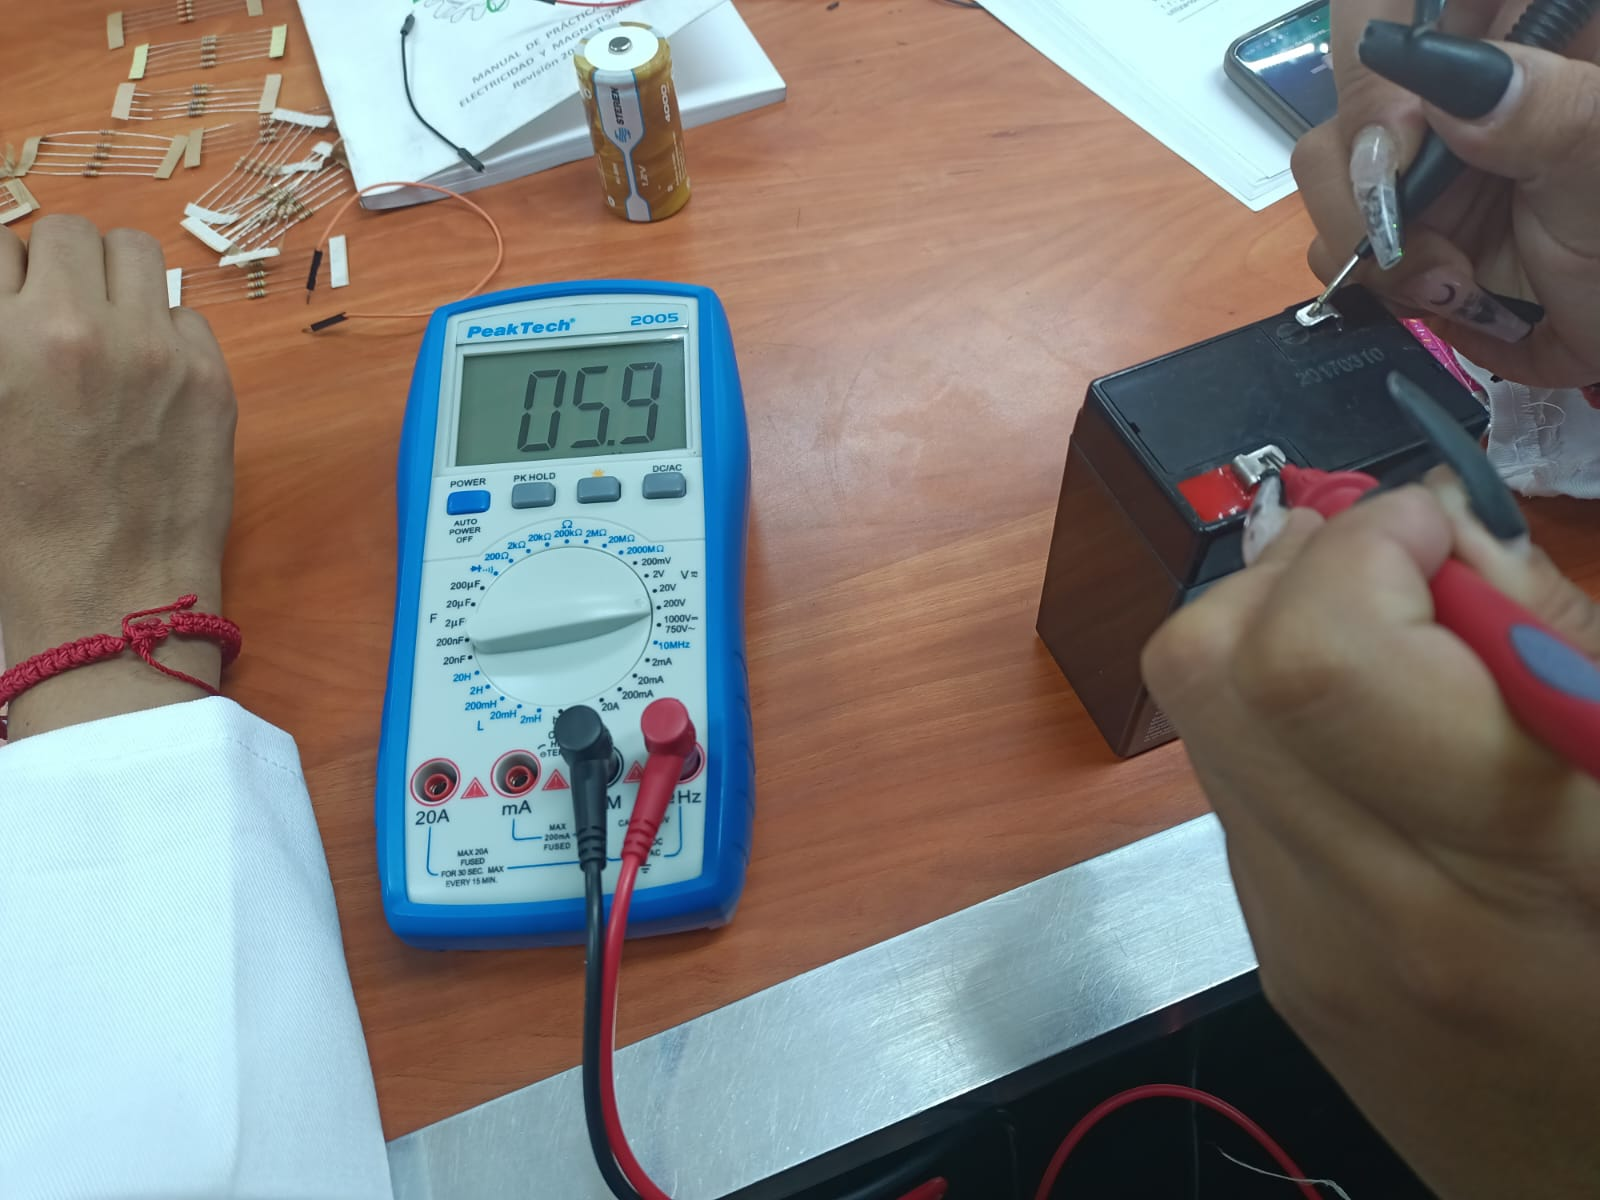
\includegraphics[scale = 0.1]{Imagenes/Fotos/Acumulador.jpeg}\\
	Medida del acumulador.\\
	
\includegraphics[scale = .5]{Imagenes/Fotos/Real.PNG}\\
	El valor real de la diferencia de potencial del acumulador es de 6V.
\end{center}

 Mediciones con la fuente de poder respetando su polaridad.
 
\begin{tabular}{ p{4cm} p{3cm} }
	\hline
	Posición 0: & 0.03 volts \\
	\hline
	Posición 10: & 10.01 volts \\
	\hline
	Posición 15: & 15.52 volts \\
	\hline
\end{tabular}

 \begin{center}
	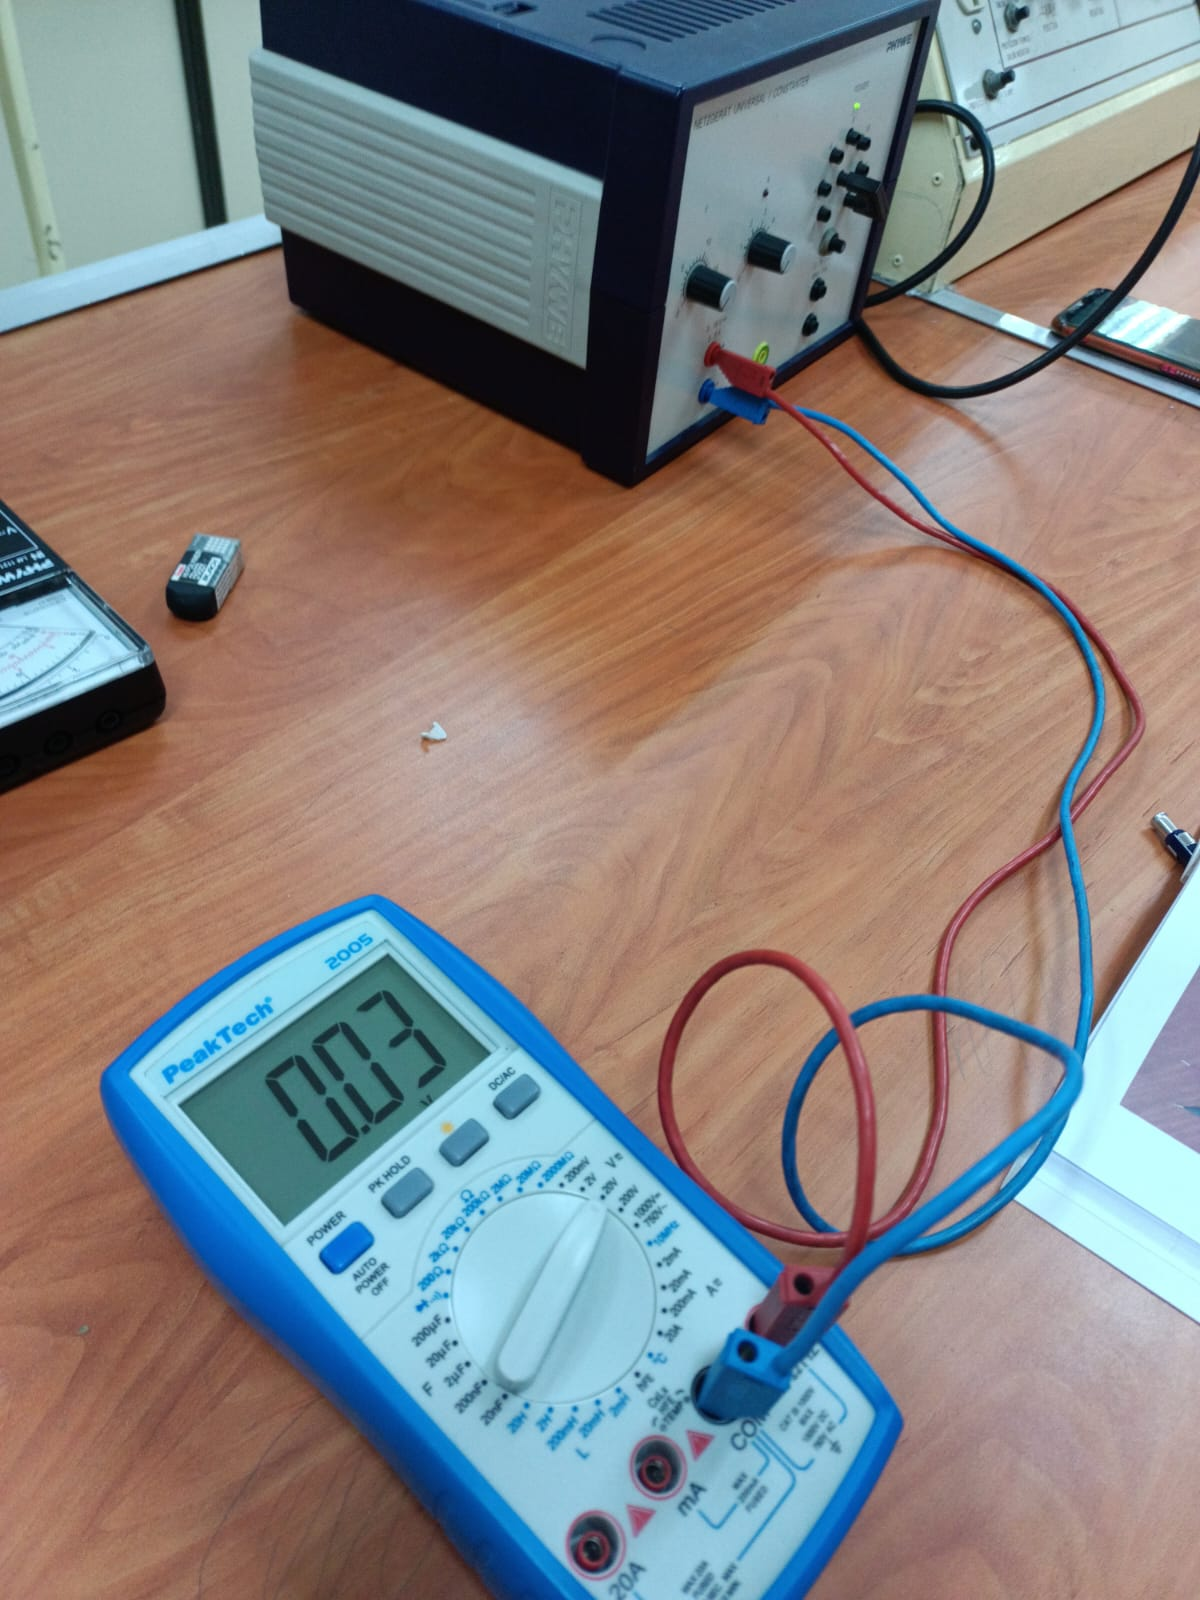
\includegraphics[scale = 0.1]{Imagenes/Fotos/Cero.jpeg}\\
	La imagen muestra la medida en la posición 0 que no tiene un valor de 0V en realidad , tiene uno de 0.03V.
	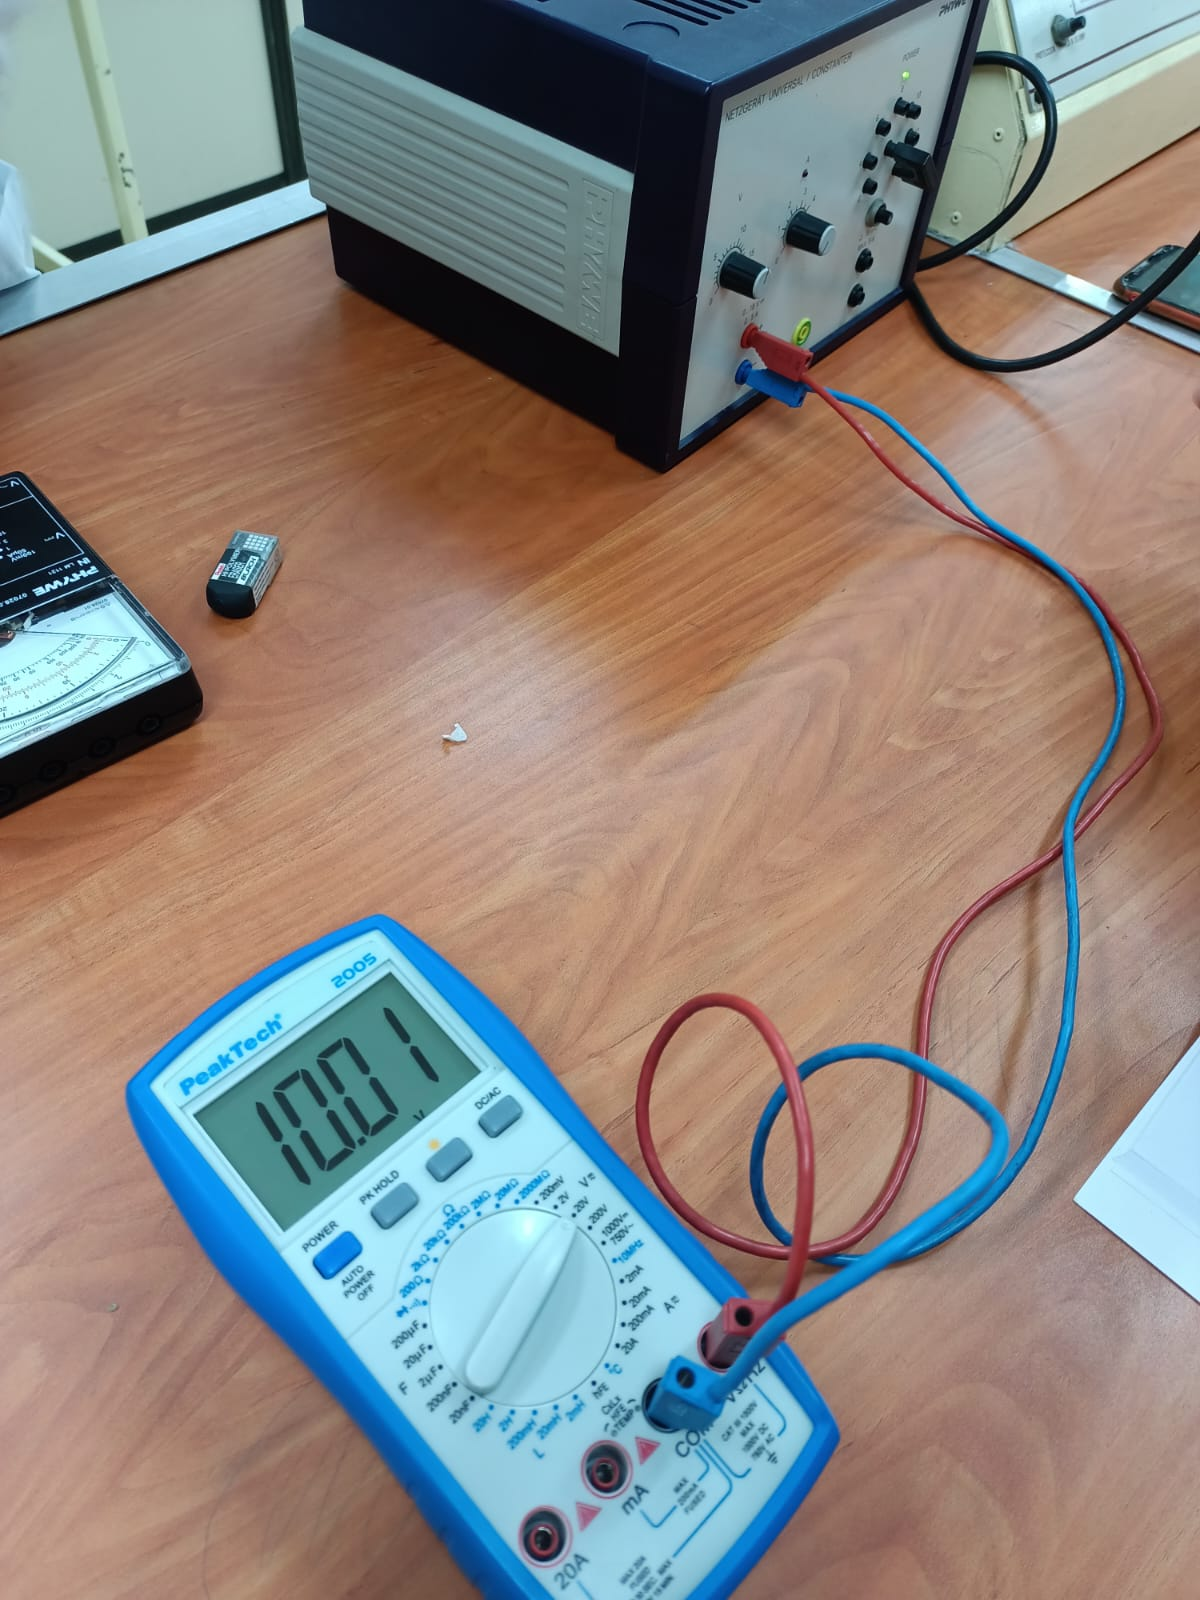
\includegraphics[scale = 0.1]{Imagenes/Fotos/Diez.jpeg}\\
	La imagen muestra el potenciometro de la fuente ajustado para que de un valor cercano a 10V tomando a consideración que el cero no es cero.
	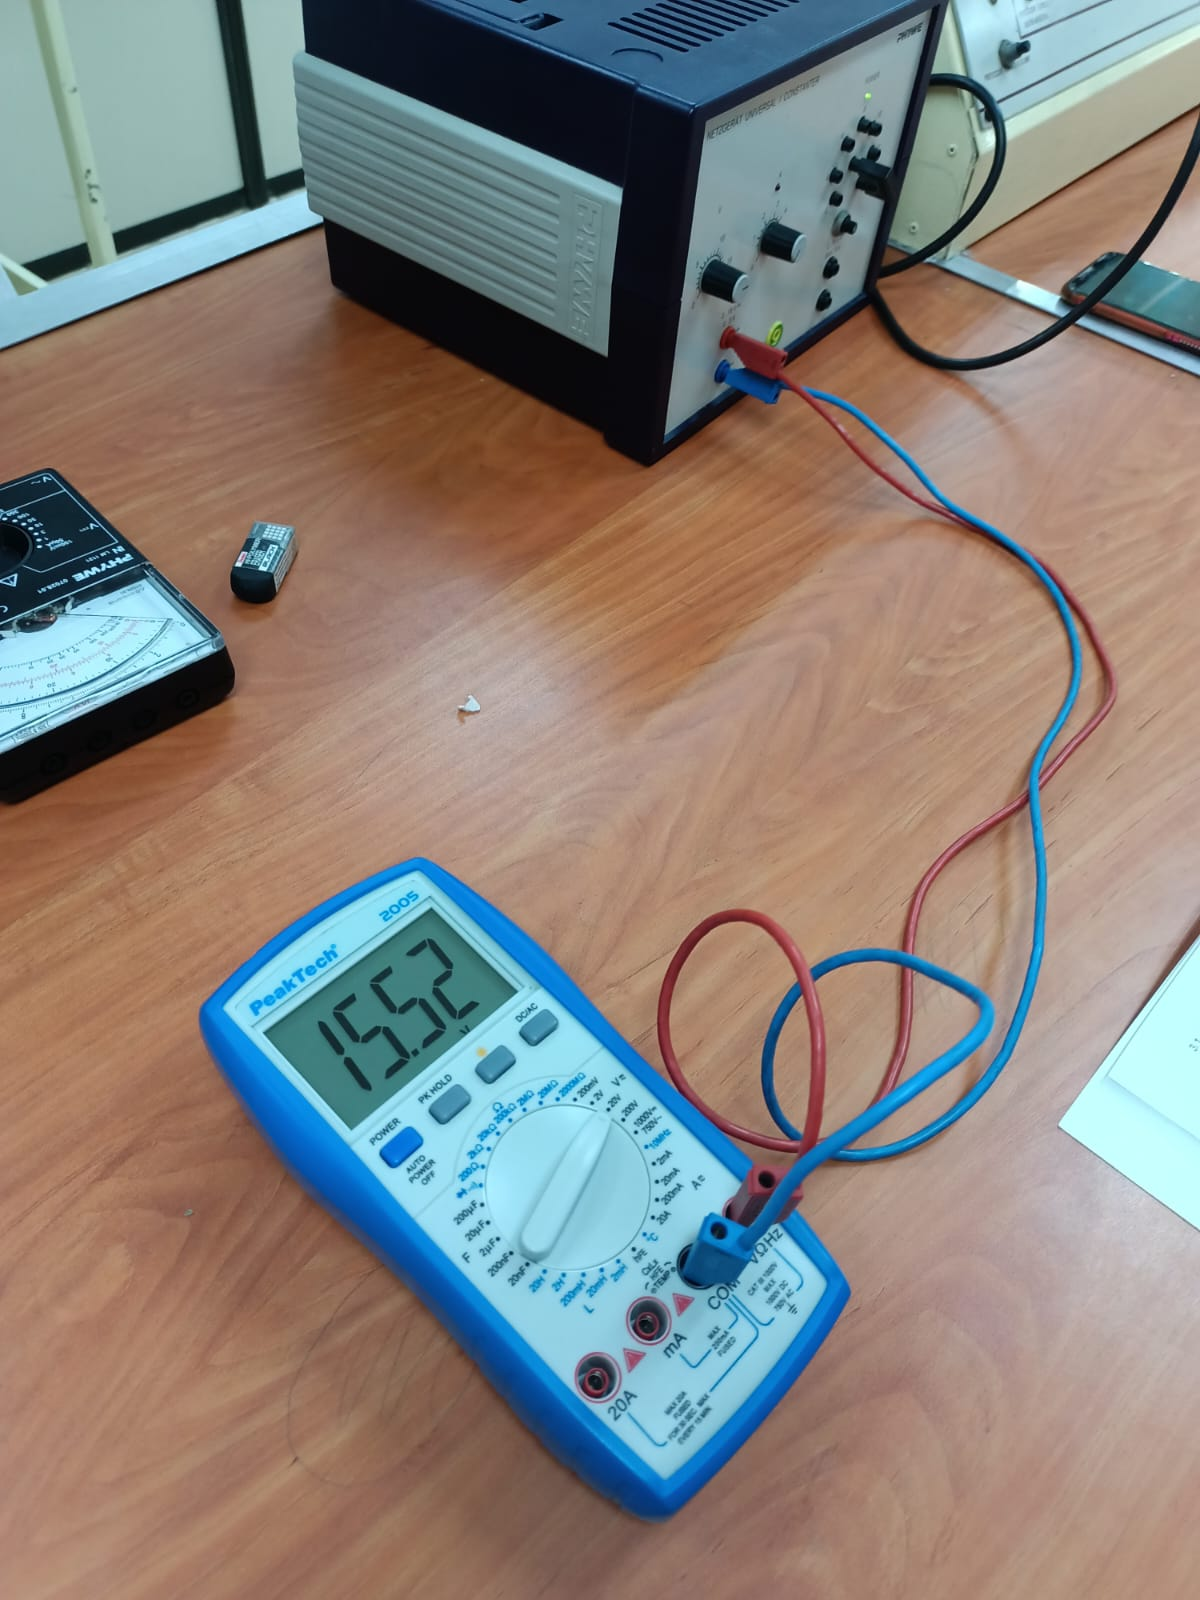
\includegraphics[scale = 0.1]{Imagenes/Fotos/Quince.jpeg}\\
	La imagen muestra la medida obtenida justo en la posición 15, nuevamente, se observa una variación.
 \end{center}

 Es importante verificar cuando se utiliza una fuente de poder regulable, que esta esté bien calibrada y si no lo está, considerar el rango de inexactitud que posee para evitar dañar nuestros circuitos.
\subsection{Mediciones de diferencia de potencial eléctrico de corriente alterna(vóltmetro).}

\begin{tabular}{ p{4cm} p{3cm} }
	\hline
	Posición 12: & 125.6 volts \\
	\hline
	Posición 13: & 0.1 volts \\
	\hline
	Posición 23: & 14 volts \\
	\hline
\end{tabular}

\begin{center}
	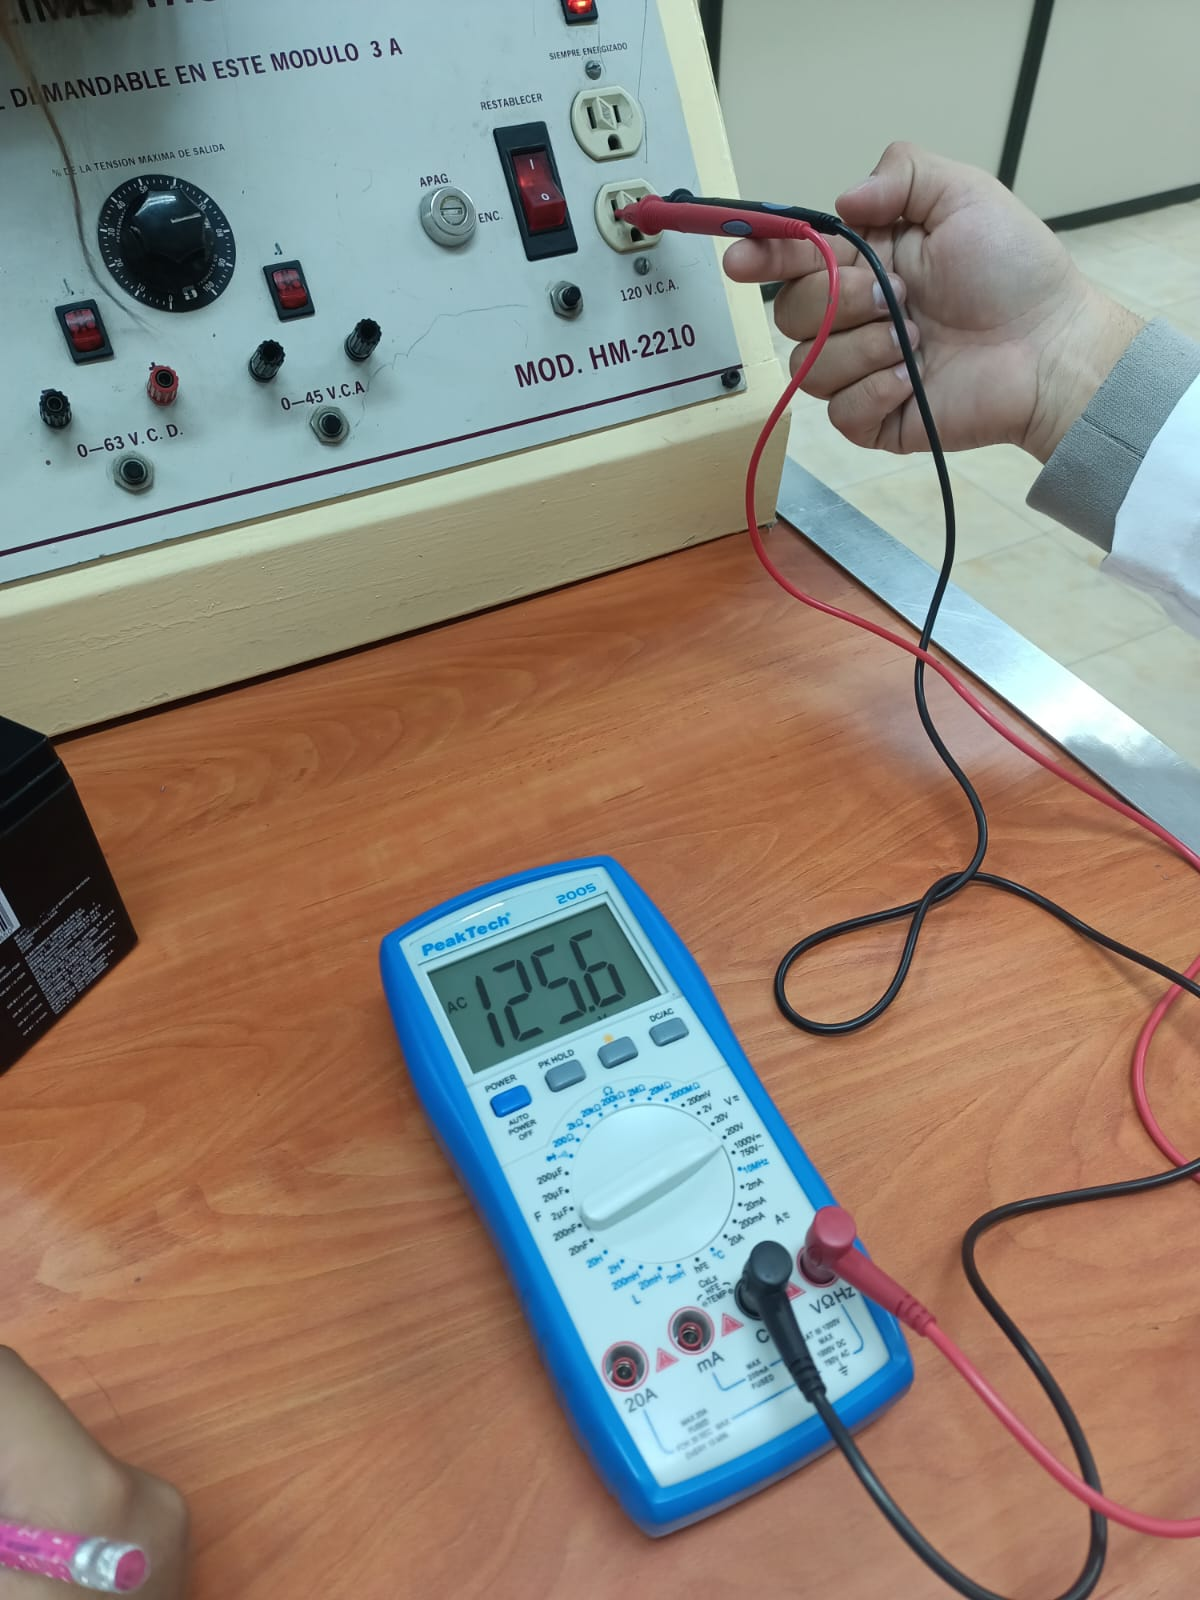
\includegraphics[scale = 0.1]{Imagenes/Fotos/12.jpeg}\\
	Diferencia de potencial eléctrico en la posición 12.
	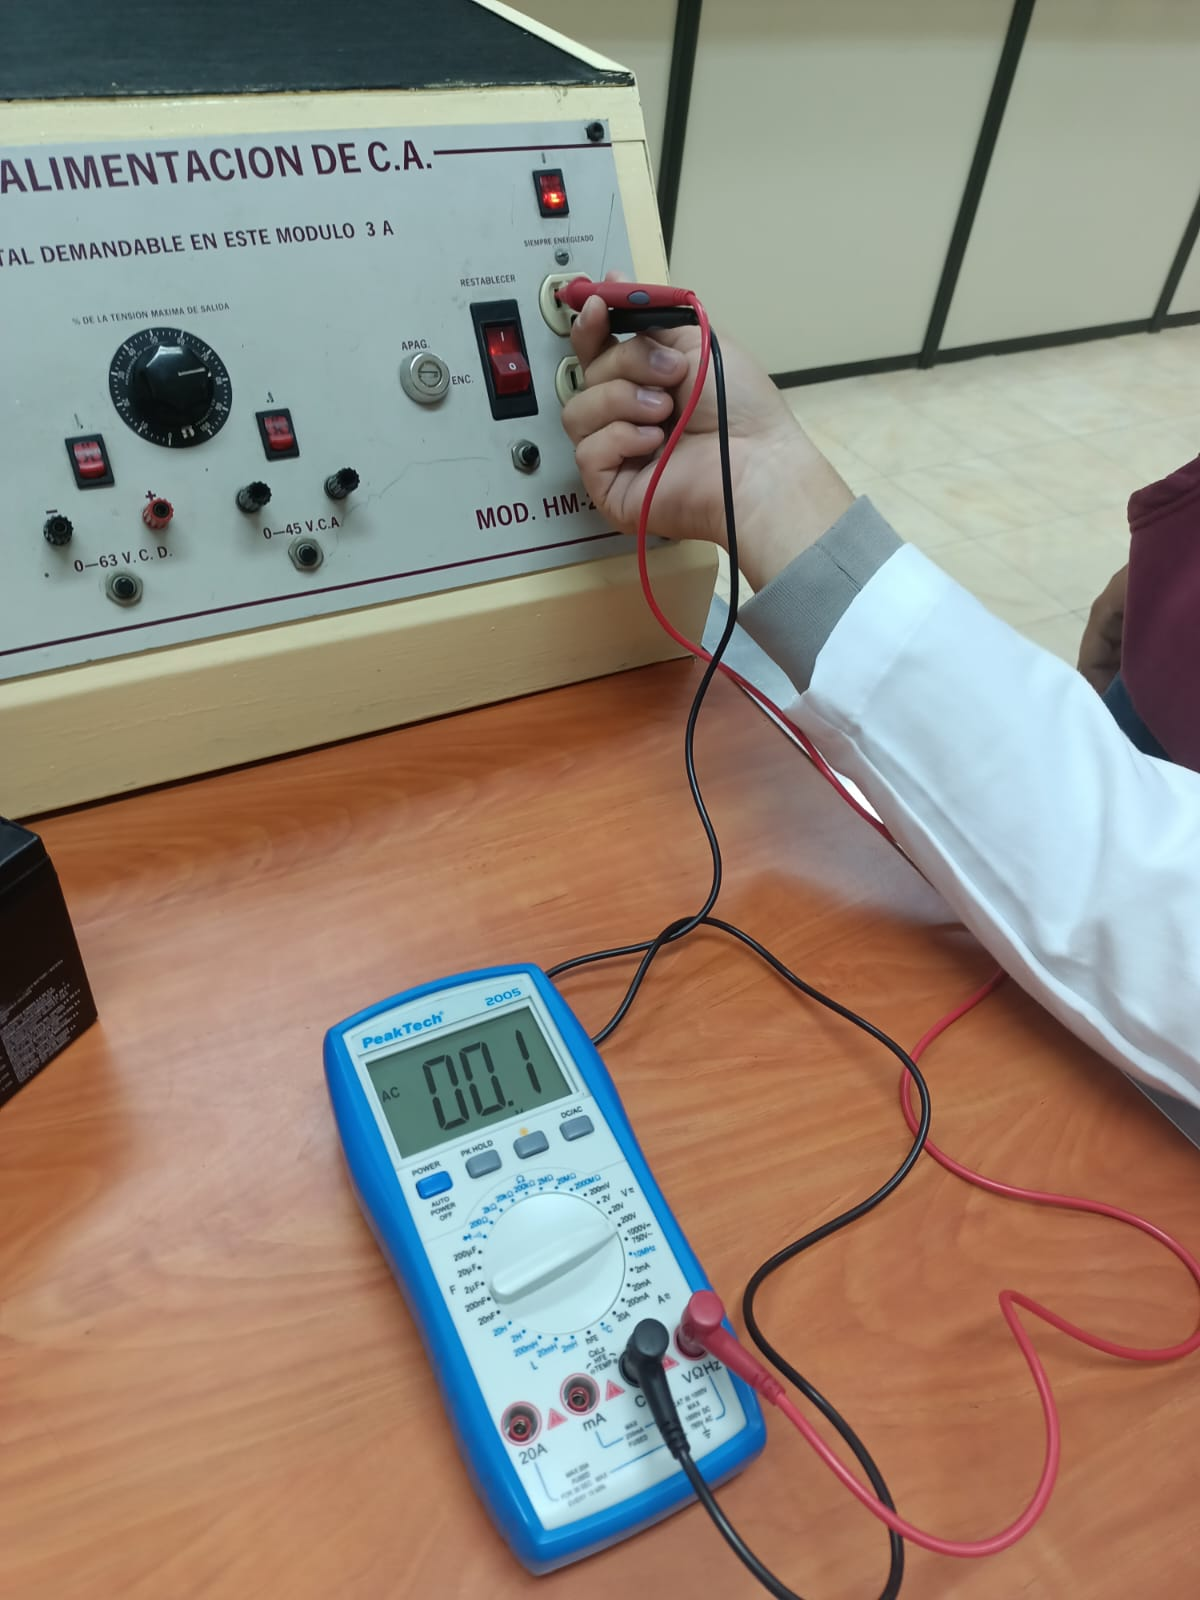
\includegraphics[scale = 0.1]{Imagenes/Fotos/13.jpeg}\\
	Diferencia de potencial eléctrico en la posición 13.	
	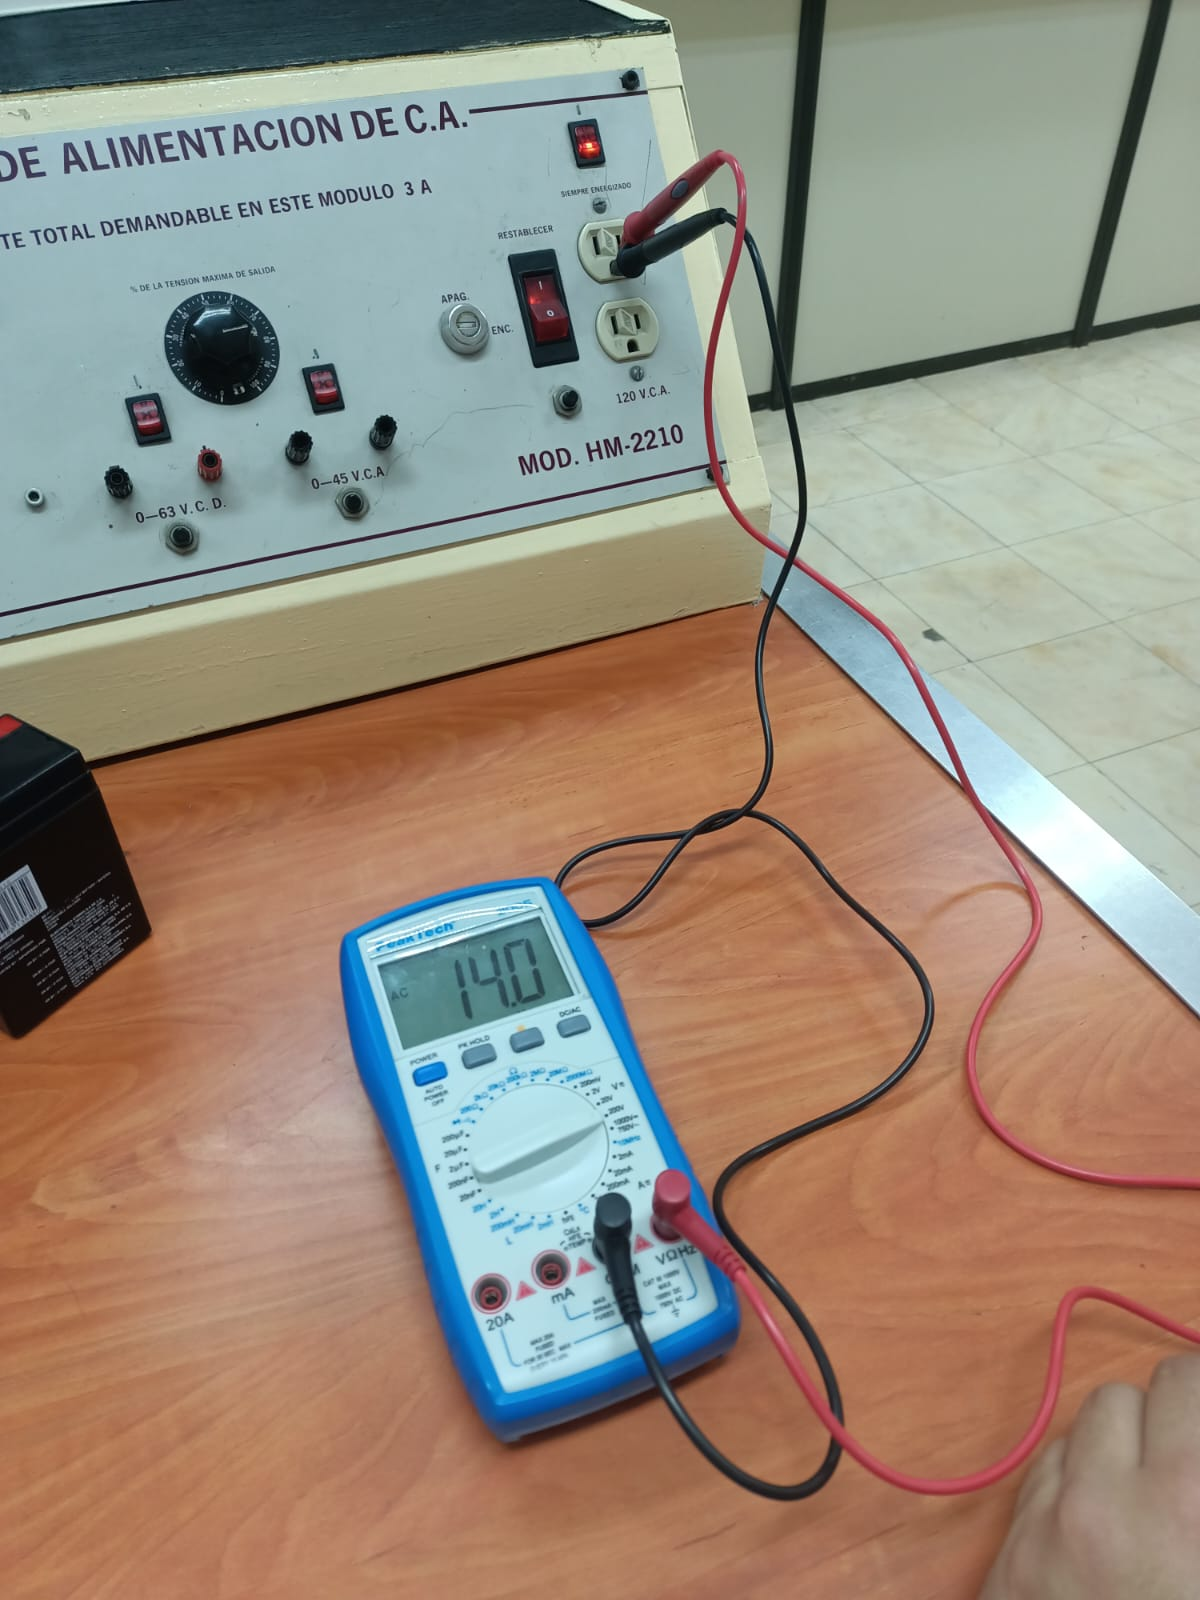
\includegraphics[scale = 0.1]{Imagenes/Fotos/23.jpeg}\\
	Diferencia de potencial eléctrico en la posición 23.
\end{center}
 
La medida normal entre fase y neutro es de entre 100V a 127 V. Con ello sabemos que la posición 1 y 2 , una de ellas es el neutro y la otra la fase. Por descarte , la de abajo es la tierra (3).
La medida entre fase y tierra es un número pequeño a comparación de fase y neutro, mientras que entre neutro y tierra debe ser cercano a 0. Con ello se establece que el contacto de la izquierda (1) es el neutro y el de la derecha la fase(2).

\subsection{Mediciones de intensidad de corriente directa(amperímetro).}

\begin{tabular}{ p{4cm} p{3cm} }
	\hline
	$I_(cd)$: & 85.5 mA \\
	\hline
\end{tabular}

\begin{center}
	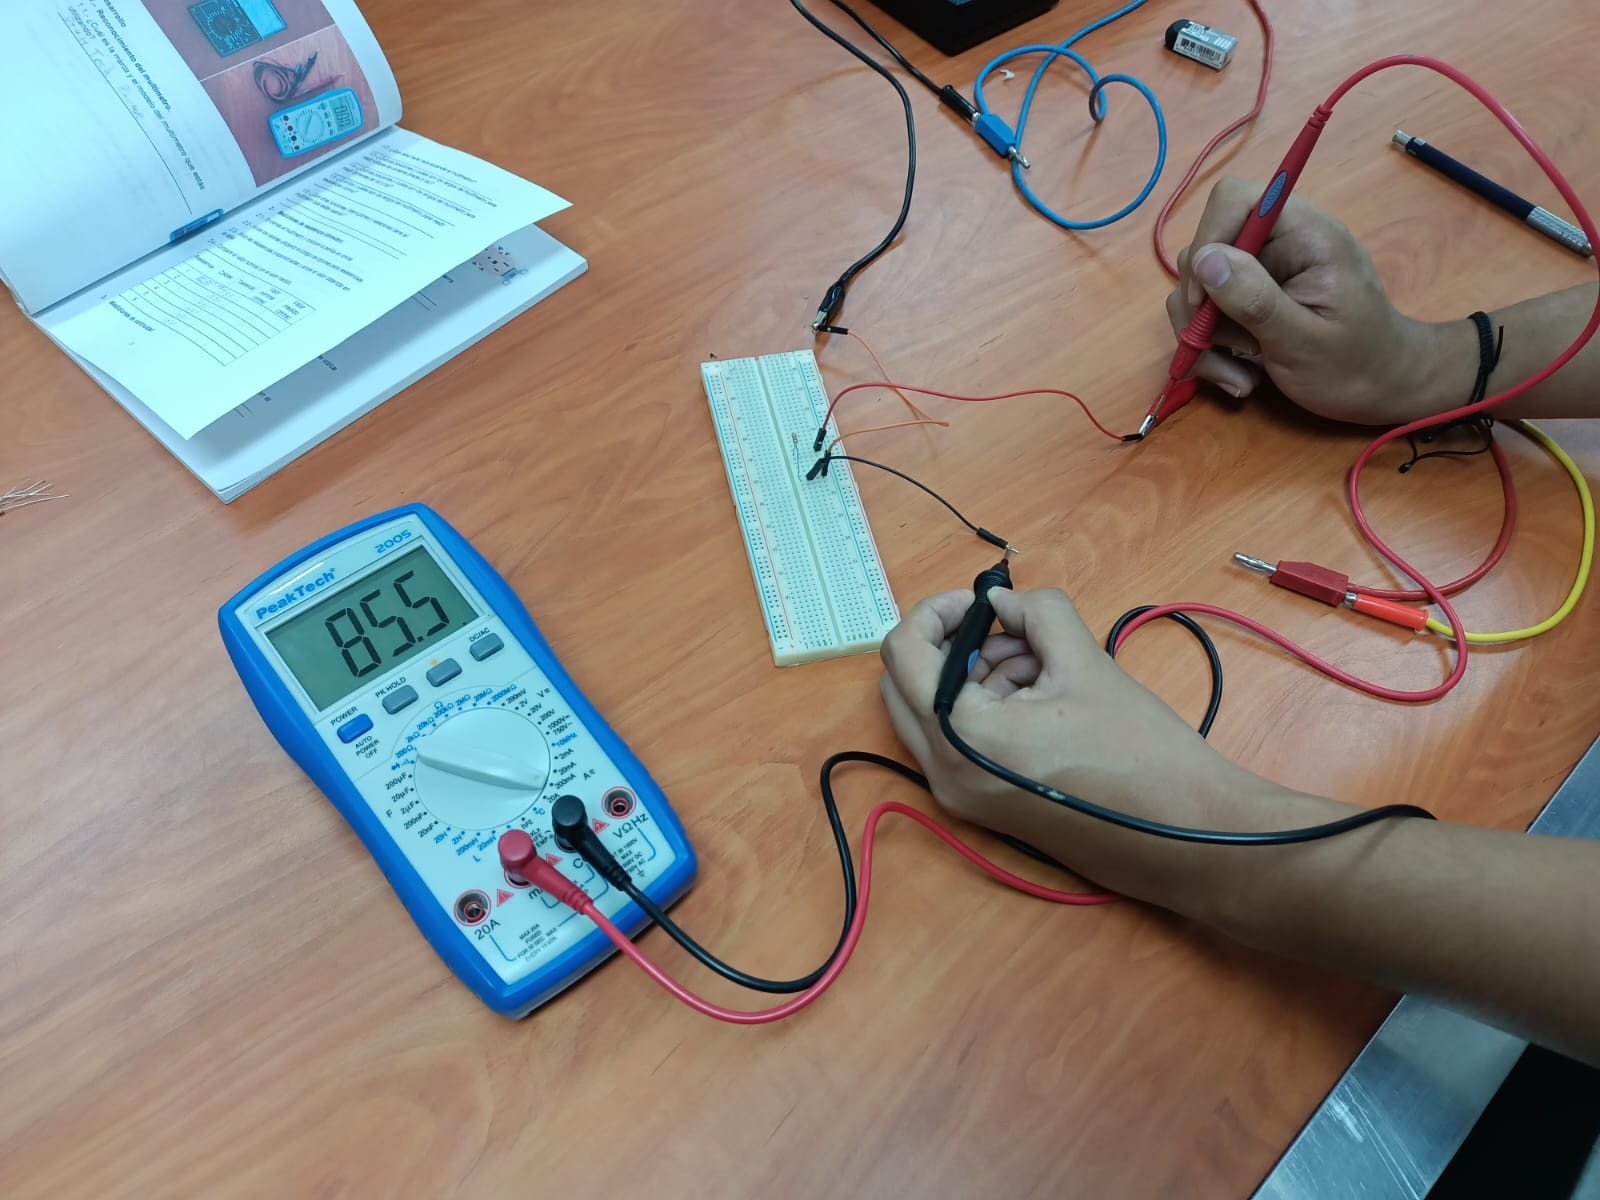
\includegraphics[scale = 0.1]{Imagenes/Fotos/Reina.jpeg}\\
	Medida de intensidad de corriente directa, magnitud obtenida 85.5 mA (0.0855A)
\end{center}
El valor teórico de corriente eléctrica según la ley de Ohm ese establece de la siguiente manera.


	$V = I \cdot R \implies  I = \frac{V}{R} = \frac{10V}{1000\Omega()} = 0.01 \frac{\cancel{V}}{\frac{\cancel{V}}{A}} = 0.01A$ 

La diferencia entre el valor teórico y el valor real es de 0.0755 A, esto es por causa de una variación en el valor nominal del resistor y que la fuente a pesar de estar en la posición de 10 V , no envía exactamente 10V.

\section{Conclusiones.}

\subsection*{Daniela Elizabeth Pérez Vargas.}
Durante esta práctica la medición de diferencia de potencial eléctrico que se hizo nos permitió determinar la diferencia de Diferencia de potencial eléctrico entre dos puntos de un circuito. 
Al realizar estas mediciones de diferencia de potencial eléctrico, se pudo observar las mediciones de diferencia de potencial eléctrico que  permitieron determinar la energía eléctrica presente en un circuito, la polaridad de los componentes, el estado de carga de las baterías y la calidad de la corriente eléctrica suministrada por una fuente de alimentación. Se utilizó  instrumentos como multímetros o voltímetros, Estos dispositivos nos ayudaron para proporcionar mediciones precisas, y conocer las diferentes variaciones durante los diferentes experimentos, al aumentar el número de partículas también aumenta la energía potencial correspondiente a cada una de ellas y por tanto también aumenta el diferencia de potencial eléctrico, es decir en algunos era constante. 
\subsection*{Jesús Martinez Amac.}
En conclusión, las mediciones de diferencia de potencial eléctrico nos permiten garantizar un funcionamiento adecuado de los dispositivos eléctricos y electrónicos, así como para diagnosticar problemas o fallas en los sistemas.
Al realizar mediciones de diferencia de potencial eléctrico nos dimos cuenta de las variaciones entre polaridades de cada experimento y la precisión con la que medimos se reflejan con más precisión el valor real del diferencia de potencial eléctrico.
 Si el diferencia de potencial eléctrico a medir se encuentra fuera del rango seleccionado, se debe ajustar al rango o utilizar un equipo de medición con un rango más amplio.
En resumen, las mediciones de diferencia de potencial eléctrico son cruciales para el análisis y diagnóstico de los sistemas eléctricos y electrónicos. Al realizar estas mediciones, se debe prestar atención a la precisión, seguridad, rango de medición y condiciones ambientales, para obtener resultados confiables y precisos como los de esta práctica.
\subsection*{José Emilio Hernández Huerta.}
<<<<<<< HEAD
En esta practica con los diferentes tipos de medición que hicimos llegamos a diferentes conclusiones, la primera antes de la existencia de multímetros existían herramientas de medición como el voltímetro especializado en medir el potencial eléctrico, el amperímetro para medir el amperaje de los circuitos eléctricos, entre otros más. Con la llegada del multímetro todo esto se juntó ayudando a mejorar las mediciones con solo un aparato de medición. Al igual que me deja con dudas como: ¿Cómo funcionan?, ¿Qué hacen los automáticos para saber solos el rango de medidas?, etc. Otra de las cosas que puede medir el multímetro es la temperatura y la frecuencia, ambas generándome intriga por saber de la misma forma como funcionan. Yo solo espero las prácticas de electrónica para poder emplear los conocimientos adquiridos en esta practica en un ambiente un poco mas cercano a la realidad. 
=======
En esta practica con los diferentes tipos de medición que hicimos llegamos a diferentes conclusiones, la primera antes de la existencia de multímetros existían herramientas de medición como el voltímetro especializado en medir el Diferencia de potencial eléctrico, el amperímetro para medir el amperaje de los circuitos eléctricos, entre otros más. Con la llegada del multímetro todo esto se juntó ayudando a mejorar las mediciones con solo un aparato de medición. Al igual que me deja con dudas como: ¿Cómo funcionan?, ¿Qué hacen los automáticos para saber solos el rango de medidas?, etc. Otra de las cosas que puede medir el multímetro es la temperatura y la frecuencia, ambas generándome intriga por saber de la misma forma como funcionan. Yo solo espero las prácticas de electrónica para poder emplear los conocimientos adquiridos en esta practica en un ambiente un poco mas cercano a la realidad. 
>>>>>>> 05e24634aa0090a7e477c33ffea4fc7ff62d4b5e
\subsection*{Nataly Bejarano Garduño.}

En esta práctica vimos que el multímetro es fundamental para realizar mediciones de carga eléctrica en los circuitos, A su vez en esta práctica pudimos observar las funciones de medición de continuidad, diferencial de potencial, resistencias y corriente 
Nos percatamos que la diferencia de potencial eléctrico determina la energía eléctrica que hay en el circuito, también su polaridad y la cantidad de corriente eléctrica dada por la fuente de alimentación. 
Cada uno de los experimentos nos permitieron darnos cuenta que no existen valores negativos en las mediciones, y que antes de usar el multímetro necesitamos conocer su funcionamiento para usar de manera correcta. 
En conclusión las mediciones de diferencia de potencial eléctrico son muy importantes para analizar los sistemas eléctricos y es importante prestar mucha atención para que los resultados sean correctos y haya un margen de error muy bajo
\subsection*{Uriel Grimaldi Díaz.}
El uso del multímetro es fundamental para realizar mediciones de magnitudes eléctricas en diferentes circuitos. Durante la práctica, se enfatizó en las funciones de medición de resistencia, continuidad, diferencia de potencial eléctrico (en corriente directa y corriente alterna) y corriente. El multímetro, ya sea digital o analógico, ofrece diversas opciones de medición y utilidades relacionadas con el análisis de circuitos electrónicos. Antes de utilizar el multímetro, es necesario realizar comprobaciones de rutina, como verificar la carga de la batería y la integridad de las puntas de medición. 
Para medir la diferencia de potencial eléctrico, corriente y resistencia, se deben seguir las recomendaciones específicas y seleccionar el rango adecuado en el multímetro. Además, se aplicó la Ley de Ohm, que establece la relación entre la diferencia de potencial eléctrico, la corriente y la resistencia en un circuito electrónico. Otra aspecto importante que aplicamos fue el uso del código de colores en los resistores, el cual nos proporciona información sobre el valor nominal de la resistencia y compararlo con su valor real.
En el desarrollo experimental, se llevaron a cabo mediciones de resistencia utilizando el óhmetro del multímetro y se compararon los valores nominales y los valores medidos. También se realizaron mediciones de continuidad y se identificó la estructura de una protoboard. Para las mediciones de diferencia de potencial eléctrico, se utilizaron tanto una pila, un acumulador y una fuente regulada, y se registraron los valores obtenidos, además de saber diferenciar entre estos tres tipos de fuentes. Asimismo, se realizaron mediciones de diferencia de potencial eléctrico de corriente alterna y se identificaron los contactos de fase, neutro y tierra física.
En resumen, el uso adecuado del multímetro y la comprensión de sus funciones son esenciales para realizar mediciones precisas en circuitos eléctricos. El conocimiento de la Ley de Ohm y el código de colores en los resistores complementan la comprensión teórica de las mediciones eléctricas. A través de la práctica experimental, se pudo aplicar estos conocimientos y obtener resultados medibles para diferentes magnitudes eléctricas además de poder interpretar los mismos.
\begin{thebibliography}{0}
	\bibitem{citekey}[Bragado, I. M. (2003). Física General.]
	\bibitem{citekey}[Benchimol, D. (c. 2020). Electrónica práctica. USERSHOP.]
	\bibitem{citekey}[Peaktech. (2016). Manual de Usuario Peaktech 2005.]
		
\end{thebibliography}

\end{multicols}

\end{document}
